\documentclass[review]{elsarticle}

\usepackage{lineno,hyperref}
\modulolinenumbers[5]
\journal{Epidemics}

\usepackage{amsmath,amssymb,amsthm}
\usepackage{graphicx}
\usepackage{booktabs}
\usepackage{tikz}
\usetikzlibrary{shapes.geometric, arrows.meta, positioning, calc, backgrounds, fit, shadows}

\theoremstyle{plain}
\newtheorem{theorem}{Theorem}
\newtheorem*{theorem5R}{Theorem 5R}  % Custom environment to avoid auto-numbering
\newtheorem{lemma}{Lemma}
\newtheorem{corollary}[theorem]{Corollary}
\theoremstyle{definition}
\newtheorem{definition}{Definition}

\definecolor{navyMain}{RGB}{24, 48, 89}
\definecolor{tealMain}{RGB}{16, 124, 138}
\definecolor{coralMain}{RGB}{210, 85, 40}
\definecolor{slateGray}{RGB}{65, 80, 100}
\definecolor{cardTealBg}{RGB}{242, 251, 252}
\definecolor{cardBlueBg}{RGB}{243, 247, 254}
\definecolor{cardOrangeBg}{RGB}{255, 247, 242}
\definecolor{cardGrayBg}{RGB}{248, 250, 253}
\definecolor{panelBorderBlue}{RGB}{175, 200, 230}
\definecolor{panelBorderOrange}{RGB}{245, 190, 160}

\begin{document}

\begin{frontmatter}

\title{The Predictability Horizon of Epidemic Forecasts: Why Near-Threshold Forecasts Fail and How Much Data They Need}

\author[inst1]{Author Name\corref{cor1}}
\ead{author@institution.edu}
\cortext[cor1]{Corresponding author}

\affiliation[inst1]{organization={Department of Infectious Disease Epidemiology, Public Health Research Institute},
                    city={City},
                    postcode={00000},
                    country={Country}}

\begin{abstract}
Epidemic forecasting systematically deteriorates near the transmission threshold, presenting a long-standing challenge for computational epidemiology and public health preparedness. While operational failures are commonly attributed to data scarcity or algorithmic limitations, a mechanistic theoretical characterization of fundamental predictability limits derived from underlying data-generating processes and information-theoretic blind zones has remained elusive. Here, we establish a theoretical framework for epidemic predictability limits derived from the negative-binomial branching process. By performing an exact orthogonal decomposition of relative forecast mean squared error into an irreducible demographic stochasticity floor and an exponentially compounding parameter-uncertainty term, we derive a closed-form predictability horizon formula linking reproduction number signal-to-noise ratio, outbreak scale, offspring overdispersion, and target accuracy, providing order-of-magnitude empirical support through high-throughput stochastic simulations.

Addressing the core mechanisms of predictability limits, our theoretical and empirical analyses yield four principal findings. First, under the negative-binomial likelihood, we establish the Cram\'er--Rao identification bound and prove that resolving whether an outbreak is in a supercritical growth state requires a strict cumulative case count threshold, below which no estimator can reliably determine the direction of transmission. Second, we characterize the near-critical finite-population window where quasi-stationary long-tailed fluctuations cause relative forecast error to become of the same order as the mean itself, triggering a structural collapse of the predictability horizon. Third, we derive a scale-invariant logarithmic variance floor of order $1/k$ for macro-aggregated incidence along with persistent growth-rate variance accumulation, quantitatively explaining observed empirical variance scaling behavior in surveillance data. Fourth, machine-learning benchmarks demonstrate that, under designated likelihood and information sets, flexible gradient boosting models saturate the theoretical error floor but cannot surpass asymptotically optimal unbiased maximum likelihood and Cram\'er--Rao bounds; a five-component prospective error budget on real-world surveillance data further reveals that short-horizon forecast failures are overwhelmingly driven by exogenous transmission shifts and model structure misspecification rather than parameter estimation noise. These findings establish near-threshold forecast degradation as an intrinsic physical and statistical constraint. Operational forecasting hubs should compute and pre-register predictability horizons ex ante, transitioning surveillance strategy from forcing low-confidence projections in blind zones to active vigilance and targeted resource reallocation.
\end{abstract}

\begin{keyword}
Epidemic forecasting \sep Predictability horizon \sep Branching processes \sep Cram\'er--Rao lower bound \sep Demographic stochasticity \sep Near-critical dynamics \sep Information-theoretic limit \sep Model misspecification
\end{keyword}

\end{frontmatter}

\linenumbers

\section{Introduction}

Epidemic forecasting exhibits sharp phase transitions: forecasts of established waves often succeed weeks ahead, while forecasts near the transmission threshold routinely fail \citep{scarpino2019predictability, reich2019collaborative}. This pattern has been attributed to model limitations or data scarcity, yet growing evidence points to intrinsic constraints \citep{farrow2017information, perofsky2017forecasting}. Collaborative forecasting hubs for influenza, dengue, and COVID-19 \citep{mcgowan2019collaborative, johansson2019open, cramer2022evaluation} have made this failure pattern visible at scale, and systematic evaluation frameworks \citep{bracher2021evaluating} now quantify it routinely, yet the underlying boundary between achievable and unachievable accuracy has not been analytically derived from underlying transmission dynamics. The broader forecasting literature has repeatedly reached the same qualitative conclusion by empirical comparison rather than derivation: real-time Bayesian and likelihood-based estimators of early growth rate are most informative, and least reliable, in the earliest and near-threshold stages of an outbreak \citep{bettencourt2008real, white2008likelihood, fraser2007estimating}; semi-mechanistic and probabilistic forecasting frameworks built for operational use routinely report degraded skill in exactly these regimes \citep{funk2018realtime, held2017probabilistic}; and the RAPIDD Ebola forecasting challenge, a systematic multi-team comparison, found that no participating model reliably outperformed a naive baseline during the low-incidence, near-extinction phase of the outbreak \citep{viboud2018rapidd}. A review of real-time forecasting practice during the 2014--2016 West African Ebola epidemic and subsequent outbreaks likewise identified near-threshold and small-outbreak regimes as a persistent, cross-cutting source of forecast failure independent of the modeling framework used \citep{desai2019realtime}.

Near the epidemic threshold, parameter estimation itself is known to be biased and unstable \citep{britton2019estimation}, compounding the demographic stochasticity intrinsic to the classical branching and compartmental description of epidemic growth \citep{kermack1927contribution}. This connects to a long-standing question in disease ecology and statistical physics: whether sharp thresholds for invasion or persistence should be expected at all in finite, stochastic host populations \citep{lloydsmith2005should}, and how the critical behavior of the underlying stochastic process\textemdash formally analogous to dynamical percolation near a critical point\citep{grassberger1983critical}\textemdash shapes the achievable precision of any forecast built on top of it. Despite this accumulated empirical and theoretical evidence that near-critical dynamics are qualitatively different from supercritical ones, no closed-form expression currently ties the reproduction number $R$, the offspring dispersion $k$, the outbreak scale, and parameter uncertainty directly to a quantitative forecasting horizon.

The absence of such a theory creates a practical problem for operational forecasting systems. When a real-time forecast fails\textemdash predicting continued exponential growth that instead plateaus, or declaring an outbreak over when it resurges\textemdash the failure could be attributed to model misspecification, insufficient data, or structural unidentifiability inherent to the epidemiological process itself. Without a principled decomposition of forecast error into these components, forecasting teams face an unsolvable attribution problem: should resources be invested in more sophisticated models, expanded surveillance, or acceptance that the current outbreak phase is simply not forecastable at the desired accuracy? This ambiguity has practical consequences for public communication as well. Forecasts issued during inherently unforecastable phases\textemdash such as the near-critical window characterized in our Theorem 3\textemdash erode public trust when they inevitably fail, yet there is currently no standard framework for flagging such phases prospectively. Our work provides this missing framework by deriving, for each outbreak phase, the minimum achievable forecast error as a function of $R$, $k$, $I_0$, and $\delta R$, and by characterizing the horizon $h^*$ beyond which no further improvement in model sophistication can be expected to yield better forecasts under the stated process assumptions.

This raises the central question: which portion of forecast error is information-theoretically unavoidable, determined solely by the epidemiological process\textemdash reproduction number $R$, dispersion $k$, initial scale $I_0$, parameter precision $\delta R$, and reporting mechanism\textemdash and can the boundary be expressed in closed form? Unlike empirical model-comparison studies, which characterize \emph{which} methods fail near threshold, this work characterizes \emph{why}: the minimum achievable forecast error at each horizon is derived from the generative stochastic process alone, independent of the estimator used. This reframes near-threshold forecast failure from a methodological shortcoming to be fixed by better models into a structural property of the epidemiological process itself, with direct consequences for how forecasting resources and public communication should be allocated across outbreak phases. We answer with five theorems and one extension, all verified by simulation: Theorem 1 gives the exact decomposition of forecast error into demographic and parameter components and derives the horizon $h^*$ in closed form; Theorem 2 shows relative accuracy decays monotonically with lead time, so no forecast meets the target once the shortest useful horizon exceeds it; Theorem 3 examines the near-critical finite-population window where quasi-stationary dynamics dominate and error is set by population size rather than model sophistication; Theorem 4 establishes a likelihood-specific identification floor quantifying how much data is required to resolve $R>1$; Theorems 5 and 5R relax constant-$R$ to time-varying and persistent-drift settings. The primary theoretical contribution of this work is to establish a rigorous, generative-mechanism-based mathematical framework governing the fundamental limits of epidemic forecasting. Specifically, we derive the first exact orthogonal decomposition of relative forecast mean squared error into an irreducible demographic stochasticity floor and an exponentially compounding parameter estimation term, and resolve this balance into the first closed-form analytical predictability horizon equation $h^*(R, k, I_0, \delta R, \tau)$ in the epidemiological literature. By rigorously connecting multi-generational branching stochasticity, Cram\'er--Rao Fisher information limits, and finite-population quasi-stationary phase transitions, this framework transforms scattered empirical observations into testable, closed-form physical laws that serve as an ex-ante benchmark of forecast capability and a quantitative basis for public health resource allocation. This integration converts scattered classical results into one quantity directly usable in surveillance decisions, which neither the branching-process literature (focused on parameter estimation) nor the forecasting literature (focused on method comparison) has provided. The integrative increment can be assessed by three testable claims: (i) joint sensitivity---the three noise sources (demographic stochasticity, parameter uncertainty, near-critical quasi-stationarity) enter $h^*$ simultaneously and multiply each other, so single-source analyses cannot predict the coupling; (ii) testable prediction---the closed form yields numerical $h^*$ for any specified $(R, k, I_0, \delta R)$, directly verifiable on synthetic data and real outbreaks (Section~
\ref{sec:data}), whereas classical results offer only qualitative statements; (iii) operational benchmark---$h^*$ converts ``how long a forecast can reasonably extend'' into a pre-registrable quantitative benchmark, interfacing with interval-format scoring \citep{bracher2021evaluating}. Combination per se generates no new predictive capacity; the closed form adds the capacity to compute the forecast ceiling ex ante.

The remainder of the paper develops three related questions in turn, each answered by a set of theorems and verified by simulation and real data. The first concerns the floor on forecast error: given parameter precision, how low can error be pushed? Theorems 1--2 give the exact decomposition and the closed-form horizon $h^*$. The second concerns the collapse of predictability near the threshold: Theorem 3 characterizes the quasi-stationary window and shows that the collapse is intrinsic to the generative process rather than a modeling deficiency. The third concerns data requirements and time variation: Theorem 4 gives the case-count requirement for resolving $R>1$, and Theorems 5--5R extend the decomposition to time-varying and persistent-drift settings. The Methods section derives these answers in turn; the Results section checks each against simulation, machine learning, and real data; the Discussion returns to the practical implications for forecasting centers and public communication.

\paragraph{Collaborative forecasting hubs and systematic evaluations.}
The emergence of multi-team operational forecasting hubs for influenza \citep{mcgowan2019collaborative}, dengue \citep{johansson2019open}, and COVID-19 \citep{cramer2022evaluation} has made forecast failure patterns visible at unprecedented scale. Systematic evaluation frameworks \citep{bracher2021evaluating} now routinely quantify model skill across outbreak phases and parameter regimes, consistently finding degraded performance in near-threshold and low-incidence settings \citep{scarpino2019predictability, reich2019collaborative}. Empirical studies have documented that information content in early-epidemic data is inherently limited \citep{farrow2017information, perofsky2017forecasting}, yet no prior work has derived closed-form expressions tying this limitation to the stochastic process parameters $R$, $k$, $I_0$, and $\delta R$. Our Theorem 1 provides the first such decomposition with tight empirical verification (ratios 0.99--1.03), moving from observed failure patterns to their generative causes.

\paragraph{Branching processes and renewal frameworks.}
The negative-binomial branching process \citep{harris1963branching} and its continuous-time renewal generalization \citep{jagers1975branching} are the foundation of modern epidemic modeling. Wallinga and Teunis \citep{wallinga2004different} established the discrete-generation formalism that links individual reproduction numbers to the generation-interval distribution \citep{wallinga2007generation}, extended by Cori et al.~\citep{cori2013framework} into the widely-used EpiEstim framework for real-time $R$ estimation. Recent methodological advances \citep{gostic2020practical, abbott2020epinow2} refine these estimators for operational use, but the literature has not previously characterized the \emph{irreducible} forecast error floor arising from demographic stochasticity and parameter uncertainty combined. Our Theorem 1 closes this gap by deriving the exact two-term decomposition and its horizon formula, verified against simulations across subcritical, critical, and supercritical regimes.

\paragraph{Critical phenomena and extinction dynamics.}
Near the epidemic threshold $R \approx 1$, finite populations exhibit quasi-stationary behavior \citep{nassel2001extinction} and critical slowing-down \citep{kessler2007extinction, assaf2017extinction}, formally analogous to phase transitions in statistical mechanics \citep{grassberger1983critical}. The interplay between demographic stochasticity and finite population size determines whether small introductions establish or fade \citep{lloydsmith2005should}, with extinction times scaling as $O(N^{1/2})$ at criticality \citep{doering2005extinction, ovaskainen2010stochastic}. Diffusion approximations \citep{ethier1986markov} provide the standard analytical route to these results, yet their connection to forecast accuracy has remained implicit. Our Theorem 3 makes this connection explicit: we derive the quasi-stationary distribution under logistic birth-death dynamics, compute its coefficient of variation (empirical/theoretical ratios 0.998--0.999), and link the critical window width $|\varepsilon| \sim (R+1)/N$ directly to the parameter-identification requirement of Theorem 4. This unifies the ecological literature on critical thresholds with the forecasting literature on near-threshold skill degradation.

\paragraph{Machine learning for epidemic forecasting.}
Deep-learning approaches to epidemic forecasting \citep{salinas2020deepar, colubri2019machine} and gradient-boosted models \citep{ke2017lightgbm} have demonstrated strong empirical performance in model-comparison challenges, yet their relationship to information-theoretic limits has not been characterized. Our machine-learning assessments (Section~\ref{sec:ml}) differ from prior work in two ways: first, we measure performance relative to the conditional forecast floor rather than against competing models; second, we test whether flexible estimators can break the Cram\'er-Rao bound of Theorem 4 under the assumed likelihood. We find that gradient boosting operates 1--18\% above the floor (not orders of magnitude), and that a neural estimator does not surpass the classical MLE in the idealized branching setting (bootstrap $p = 1.0$), consistent with MLE asymptotic optimality. This establishes that the bounds derived here are not artifacts of suboptimal estimation but intrinsic properties of the generative process.


\section{Methods}
\subsection{Data}\label{sec:data}


Applying the theoretical framework to national surveillance data shows what values the horizon formula takes in real outbreak settings. We emphasize that this is a method demonstration, not an empirical validation: the horizons in Table~\ref{tab:horizons} assume ideal constant-$R$ conditions and finalized (non-real-time) surveillance data, and the bootstrap confidence intervals are wide (e.g., RSV 2025--26: 34.3--134.7 weeks), reflecting substantial parameter uncertainty. Operational horizons would be further shortened by $R$ drift, reporting delays, and interventions.

We analyzed three respiratory pathogens from U.S. national surveillance:
\begin{itemize}
\item COVID-19: Weekly confirmed cases, CDC COVID Data Tracker, Jan 2021--Dec 2023.
\item RSV: Weekly hospital admissions, NREVSS and NSSP, Oct 2023--Mar 2026.
\item Influenza: Weekly ILINet positive tests, CDC FluView, Oct 2021--Mar 2025.
\end{itemize}

Reproduction-number estimation: Instantaneous $R_t$ via EpiEstim \citep{cori2013framework, thompson2019epiestim} with generation-interval means (COVID: 5.5 days; RSV: 6.0 days; influenza: 3.0 days \citep{nishiura2009generation, park2020forward, hakki2022serial}) and default serial-interval uncertainty. We use the intrinsic generation interval throughout rather than the realized (forward) interval, following the distinction established by \citet{svensson2007generation} and \citet{champredon2015intrinsic}; the two coincide in the constant-$R$ regime assumed here but diverge during rapid growth or decline.

Dispersion estimation: Short-window moment estimator $\hat{k} = \bar{I}^2 / (s^2 - \bar{I})$ on 8-week moving windows, following \citet{endo2020overdispersion, adam2020clustering}.

Observation windows: 4-week windows spanning epidemic onsets (weeks $t_0$ to $t_0+3$) yield initial $R$ and $\delta R = \text{sd}(R_{t_0:t_0+3})/\sqrt{4}$. Epidemic scale $I_0$ taken as week-$t_0$ incidence.

\subsubsection{Sensitivity of real-data estimates}

The horizons in Table~\ref{tab:horizons} are conditional on several methodological choices and data-quality assumptions, each of which introduces uncertainty beyond the bootstrap confidence intervals shown.

Generation-interval sensitivity. The mean generation interval $\mu_g$ appears linearly in the horizon formula $h^* \approx \mu_g (R/\delta R)\sqrt{\tau^2 - \text{floor}}$, so misspecification directly scales the calendar-time horizon. We adopt literature consensus values (COVID 5.5d, RSV 6.0d, influenza 3.0d \citep{nishiura2009generation, park2020forward, hakki2022serial}), but empirical estimates span $\pm 1$--2 days depending on contact-tracing methodology, variant, and setting \citep{farrow2017information, perofsky2017forecasting}. A $\pm 20\%$ error in $\mu_g$ translates to a $\pm 20\%$ error in $h^*$ measured in calendar time, though the generation-count horizon $h^* / \mu_g$ remains invariant. EpiEstim propagates serial-interval uncertainty through its Bayesian posterior for $R_t$, but this accounts only for uncertainty in the shape of the distribution, not systematic bias in the mean; when the true mean differs from the assumed value, $R_t$ estimates are shifted systematically \citep{wallinga2007generation}, biasing both $R$ and $\delta R$ in Theorem 1.

Observation-window width. We use 4-week onset windows to estimate initial $R$ and its standard deviation $\delta R$. Narrower windows (e.g., 2 weeks) reduce the risk of violating the constant-$R$ assumption but increase $\delta R$ due to smaller sample size, shortening the horizon; wider windows (e.g., 6--8 weeks) smooth short-term fluctuations but are more likely to span regime changes (e.g., behavioral response, variant emergence), invalidating the Theorem 1 independence assumption. We tested 2-week and 6-week windows on the COVID Delta and RSV 2024--25 phases: 2-week windows increased $\delta R$ by 40--60\%, reducing $h^*$ by 30--50\%; 6-week windows decreased $\delta R$ by 20--30\% but included visible trend breaks in two of nine phases, making the constant-$R$ idealization untenable. The 4-week choice balances statistical precision against structural validity.

Dispersion-estimation window. The 8-week moving window for $k$ estimation is chosen to match the shortest scale at which moment-based estimators stabilize \citep{endo2020overdispersion}. Shorter windows yield noisier $\hat{k}$ (coefficient of variation $>0.5$ at 4 weeks in low-incidence RSV phases); longer windows (12--16 weeks) smooth over real temporal variation in superspreading intensity, which can change with control measures or population mixing \citep{adam2020clustering, lloyd-smith2005superspreading}. The population-level $1/k$ floor (Section~
\ref{eq:pop_floor}) validates that our $k$ estimates produce log-variance ratios 0.98--1.03 , indicating the window is wide enough to capture stable dispersion without conflating individual-level and population-level noise sources.

Surveillance data quality. All three data streams are subject to reporting delays (1--2 weeks for COVID/influenza, $<1$ week for RSV hospital admissions), incomplete case ascertainment (testing rates vary by symptom severity, healthcare access, and public awareness), and evolving case definitions (e.g., transition from PCR-confirmed to antigen-positive reporting during COVID Omicron). These issues affect $I_0$ (the initial epidemic scale) and $R_t$ estimation in two ways. First, reporting delays introduce right-truncation bias, typically corrected by nowcasting \citep{bastos2019nowcasting}; we use finalized (non-real-time) data to avoid this, but the correction is imperfect during rapid growth. Second, incomplete ascertainment biases $R_t$ upward if testing rates increase during the observation window and downward if they decrease; EpiEstim assumes constant reporting fraction, so $R_t$ tracks the product of biological transmissibility and reporting probability \citep{gostic2020practical}. The horizons in Table~\ref{tab:horizons} should therefore be interpreted as upper bounds under ideal constant-transmission conditions, not operational forecasts; real-world horizons are shortened by time-varying ascertainment, behavioral responses, and interventions not captured in the branching-process model.



\subsection{Model and assumptions}

Deriving the closed-form error floor requires fixing the generative model. The standing assumptions (A1)--(A4) do this; the modeling framework (Figure~\ref{fig:framework}) then assembles the two error sources into the horizon; and the closing discussion relates the framework to deterministic compartmental models.

\subsubsection{Standing assumptions}

\begin{itemize}
\item[(A1)] Offspring distribution: Independent negative-binomial with mean $R$ and dispersion $k$; variance $\sigma^2 = R + R^2/k$ per generation.
\item[(A2)] Constant reproduction number: $R$ fixed over the forecasting horizon (relaxed in Theorems 5, 5R).
\item[(A3)] Generation interval: Mean $\mu_g$ time units; horizon $h$ in generation counts.
\item[(A4)] Independent parameter estimator: $\hat{R}$ independent of the epidemic realization (same-data cross-term addressed after Theorem 1).
\end{itemize}

\subsubsection{Modeling framework}

Figure~\ref{fig:framework} summarizes the two sources of forecast error and their assembly into the horizon.

We employ the discrete-time Galton-Watson branching process with negative-binomial offspring \citep{harris1963branching, jagers1975branching, lloyd-smith2005superspreading}, the continuous-time renewal equation \citep{wallinga2004different, cori2013framework}, and logistic diffusion for finite populations \citep{ethier1986markov, nassel2001extinction, kessler2007extinction, assaf2017extinction}. This branching-process formalization is the standard route to individual- and household-level reproduction-number estimation \citep{fraser2007estimating} and to early real-time Bayesian estimation of epidemic potential \citep{bettencourt2008real}, and it underlies most likelihood-based estimators of the serial interval and growth rate used operationally \citep{white2008likelihood}. Parameter estimation follows the Cori-Wallinga framework \citep{cori2013framework, gostic2020practical, abbott2020epinow2}. The relationship between the exponential growth rate and $R$ used in Theorem 5R depends on the generation-interval distribution \citep{wallinga2007generation}.

\begin{figure}[htbp]
\centering
\resizebox{0.96\textwidth}{!}{%
\begin{tikzpicture}[
    >=Stealth,
    font=\sffamily,
    card/.style={
        rectangle, rounded corners=6pt, draw=#1, fill=white, line width=1.1pt,
        inner sep=8pt, align=center, drop shadow={opacity=0.07, shadow xshift=1pt, shadow yshift=-1.5pt}
    },
    subcard/.style={
        rectangle, rounded corners=4pt, draw=#1, line width=0.8pt,
        inner sep=5pt, align=center
    },
    panel/.style={
        rectangle, rounded corners=8pt, draw=#1, line width=0.9pt, dashed, inner sep=10pt, fill opacity=0.35
    },
    arrow/.style={
        ->, line width=1.3pt
    }
]

% ==============================================================================
% 1. TIER 1: INPUT NOISE SOURCES
% ==============================================================================
\node[card=tealMain, fill=cardTealBg, text width=6.3cm] (demo) {
    \textbf{\large\color{tealMain} Demographic Stochasticity (Intrinsic)}\\[4pt]
    \footnotesize Generative mechanism: branching (offspring $\sim \text{NB}(R, k)$)\\[4pt]
    \textbf{\small Irreducible Error Floor (Lemma 2 / Theorem 1):}\\[3pt]
    $\text{CV}^2(h) = \dfrac{(1+R/k)(1-R^{-h})}{I_0(R-1)} \xrightarrow{h\to\infty} \dfrac{1+R/k}{I_0(R-1)}$
};

\node[card=navyMain, fill=cardBlueBg, text width=6.3cm, right=1.2cm of demo] (param) {
    \textbf{\large\color{navyMain} Parameter Uncertainty (Extrinsic)}\\[4pt]
    \footnotesize Surveillance inference: estimator $\hat{R} \sim \mathcal{N}(R, \delta R^2)$\\[4pt]
    \textbf{\small Geometric Amplification (Lemma 3):}\\[3pt]
    $P(h) = \dfrac{\mathbb{E}[(\hat{R}^h - R^h)^2]}{R^{2h}} \approx \left(\dfrac{h\,\delta R}{R}\right)^2$
};

% ==============================================================================
% 2. TIER 2: ORTHOGONAL ERROR DECOMPOSITION
% ==============================================================================
\node[card=slateGray, fill=cardGrayBg, text width=12.8cm, below=1.5cm of $(demo.south)!0.5!(param.south)$] (decomp) {
    \textbf{\large\color{navyMain} Orthogonal Forecast Error Decomposition (Theorems 1 \& 2)}\\[6pt]
    \Large $\text{relMSE}^2(h) = \underbrace{\text{CV}^2(h)}_{\text{\normalsize Demographic Floor}} + \underbrace{P(h)}_{\text{\normalsize Parameter Amplification}} \le \tau^2$\\[5pt]
    \small\color{slateGray} (Strictly orthogonal under branching independence; strictly monotonically increasing with horizon $h$)
};

% ==============================================================================
% 3. TIER 3: HORIZON CEILING & LIMIT THEOREMS
% ==============================================================================
\node[card=coralMain, fill=cardOrangeBg, text width=13.8cm, below=2.6cm of decomp.south] (horizon) {
    \textbf{\Large\color{coralMain} Predictability Horizons \& Fundamental Limits ($h^*$)}\\[7pt]
    
    % Two Main Horizon Formulas Side by Side with Perfect Scaling (scalebox 0.85)
    \begin{tikzpicture}[node distance=0.25cm]
        \node[subcard=coralMain, fill=white, text width=6.3cm, inner sep=4.5pt] (hmain) {
            \textbf{\small\color{coralMain} Supercritical Closed Form ($R > 1$)}\\[3pt]
            \scalebox{0.85}{$\boxed{\rule[-7pt]{0pt}{20pt}\, h^* \approx \mu_g \cdot \dfrac{R}{\delta R}\sqrt{\tau^2 - \dfrac{1+R/k}{I_0(R-1)}} \,}$}\\[3pt]
            \scriptsize ($\tau$ is target relative error tolerance)
        };
        \node[subcard=coralMain, fill=white, text width=6.3cm, inner sep=4.5pt, right=0.25cm of hmain] (hcrit) {
            \textbf{\small\color{coralMain} Near-Critical Exact Positive Root ($R \to 1$)}\\[3pt]
            \scalebox{0.85}{$\boxed{\rule[-7pt]{0pt}{20pt}\, h^*_{\text{gen}} = \dfrac{\sqrt{b^2+4\delta R^2\tau^2}-b}{2\delta R^2} \,}$}\\[3pt]
            \scriptsize (where $b = \dfrac{1+1/k}{I_0}$ is initial dispersion floor)
        };
    \end{tikzpicture}\\[8pt]
    
    % Three Columns for Sub-Theorems
    \begin{tikzpicture}[node distance=0.25cm]
        \node[subcard=coralMain, fill=white, text width=3.8cm, inner sep=4.5pt] (t3) {
            \textbf{\color{coralMain} Critical Slowing Down (Thm 3)}\\[2pt]
            \scriptsize Quasi-stationary fluctuations\\
            $|\varepsilon| \sim \frac{R+1}{N} \implies h^* \to 0$\\
            Establishment $s \approx 2\varepsilon/R$
        };
        \node[subcard=coralMain, fill=white, text width=3.8cm, inner sep=4.5pt, right=0.25cm of t3] (t4) {
            \textbf{\color{coralMain} Identification Floor (Thm 4)}\\[2pt]
            \scriptsize Cram\'er--Rao lower bound\\
            $C \ge \frac{R^2(1/R+1/k)}{\varepsilon^2} \approx 231$\\
            80\% power: $C \ge 1,428$
        };
        \node[subcard=coralMain, fill=white, text width=3.8cm, inner sep=4.5pt, right=0.25cm of t4] (t5) {
            \textbf{\color{coralMain} Real-Data Budget (Thm 5/5R)}\\[2pt]
            \scriptsize Full five-term decomposition\\
            $\text{relMSE}^2 = \text{CV}^2 + \mathcal{E}_{\text{drift}} + P$\\
            $+ \mathcal{E}_{\text{cross}} + \mathcal{E}_{\text{misspec}}$
        };
    \end{tikzpicture}
};

% ==============================================================================
% 4. CONNECTING FLOW ARROWS
% ==============================================================================
\draw[arrow, draw=tealMain] (demo.south) -- (demo.south |- decomp.north)
    node[midway, left=2pt, font=\bfseries\small\color{tealMain}] {Intrinsic contribution};

\draw[arrow, draw=navyMain] (param.south) -- (param.south |- decomp.north)
    node[midway, right=2pt, font=\bfseries\small\color{navyMain}] {Extrinsic contribution};

% Arrow from decomp to horizon with badge placed higher up
\node[fill=white, inner sep=3.5pt, rounded corners=3pt, draw=coralMain, line width=0.8pt, font=\bfseries\small\color{coralMain}, below=0.35cm of decomp.south] (critBadge) {First crossing $\text{relMSE}(h^*) = \tau$};

\draw[arrow, line width=1.8pt, draw=coralMain] (decomp.south) -- (critBadge.north);
\draw[arrow, line width=1.8pt, draw=coralMain] (critBadge.south) -- (horizon.north);

% ==============================================================================
% 5. BACKGROUND CONTAINERS
% ==============================================================================
\begin{scope}[on background layer]
    \node[panel=panelBorderBlue, fill=cardBlueBg, fit=(demo) (param), 
          label={[anchor=south west, font=\bfseries\small\color{navyMain}, xshift=4pt, yshift=2pt]north west:{\textbf{Phase I: Dual Physical Noise Sources}}}] {};
          
    \node[panel=panelBorderOrange, fill=cardOrangeBg, fit=(horizon), 
          label={[anchor=south west, font=\bfseries\small\color{coralMain}, xshift=4pt, yshift=2pt]north west:{\textbf{Phase II: Theoretical Limits \& Operational Horizons}}}] {};
\end{scope}

\end{tikzpicture}%
}
\caption{\textbf{Theoretical framework for epidemic predictability limits.} Visual summary of dual physical noise inputs (demographic stochasticity and parameter estimation noise), orthogonal mean-squared error decomposition (Theorems 1 and 2), and the derived operational horizon ceilings $h^*$ across supercritical and near-critical regimes, along with fundamental limits (Theorem 3 critical slowing down, Theorem 4 Cram\'er--Rao identification floor, and Theorems 5/5R full empirical error budget).}
\label{fig:framework}
\end{figure}

\subsubsection{Relation to deterministic compartmental models}

The negative-binomial branching process adopted here is a discrete-generation, individual-level representation of epidemic transmission. It is formally equivalent to the classical SIR and SEIR compartmental models \citep{kermack1927contribution} in the large-population limit when the generation interval is fixed and the infectious period is exponentially distributed. In that regime, the expected trajectory of a branching process with reproduction number $R$ and generation time $\mu_g$ converges to the solution of the continuous-time compartmental ODE with matched $R_0$ and mean infectious period, and the demographic stochasticity term $\text{Var}(Z_h)$ scales as $O(N)$ while the deterministic solution scales as $O(N)$, making the coefficient of variation $O(N^{-1/2})$ \citep{ethier1986markov}. For finite populations or near the threshold $R \approx 1$, the branching-process description retains demographic noise explicitly, whereas deterministic compartmental models suppress it. Our Theorems 1--2 characterize forecast error in the stochastic setting; the deterministic limit corresponds to $I_0 \to \infty$ with $\text{CV}^2(h) \to 0$, leaving only parameter uncertainty.

The discrete-generation branching model and the continuous-time renewal equation \citep{wallinga2004different} are related by the generation-interval distribution: the renewal equation
\begin{equation}
I(t) = \int_0^t I(t-s) R(t) w(s) \, ds
\end{equation}
with generation-interval density $w(s)$ reduces to the discrete branching recursion $Z_{n+1} = R \, Z_n$ (in expectation) when $w(s) = \delta(s - \mu_g)$, and the two formalisms yield identical $R$ estimates when the generation interval is correctly specified \citep{wallinga2007generation}. In the renewal framework, time-varying $R(t)$ is typically estimated via regularized inversion \citep{cori2013framework}, and the uncertainty propagation for multi-step forecasts follows the same variance-accumulation structure as Theorem 1, with the demographic floor and parameter terms both present. Our choice of the discrete branching formalism is pedagogical: it makes the two error sources algebraically separable and admits closed-form horizon expressions, whereas the renewal integral requires numerical convolution. The theoretical horizons derived here apply equally to renewal-based forecasts when the generation interval is treated as known; misspecification of $w(s)$ introduces an additional model-error term not addressed in this paper.


\subsection{Error decomposition and horizon}

 Throughout, define the relative forecast mean squared error as $\text{relMSE}^2(h) = \mathbb{E}[(I_0 \hat{R}^h - Z_h)^2]/\mathbb{E}[Z_h]^2$ (the normalized MSE of the forecast $I_0 \hat{R}^h$ against the true count $Z_h$), the squared coefficient of variation as $\text{CV}^2(h) = \text{Var}(Z_h)/\mathbb{E}[Z_h]^2$ (the demographic-stochasticity contribution), and the parameter term as $P(h; R, \delta R) = \mathbb{E}[(\hat{R}^h - R^h)^2]/R^{2h}$ (the parameter-uncertainty contribution). Theorem 1 establishes $\text{relMSE}^2(h) = \text{CV}^2(h) + P(h)$.

Relative to foundational literature, this work provides distinct incremental contributions: (i) unlike Castro et al.\citep{castro2020predictability}, who analyze Lyapunov exponents in deterministic chaotic ODEs, we derive closed-form horizons $h^*$ directly from stochastic branching processes with demographic and parameter error decomposition; (ii) unlike Parag and Donnelly\citep{parag2022fundamental}, who establish time-lag limits in real-time $R_t$ filtering, we map inference limits to forward multi-step error propagation; and (iii) unlike Drake et al.\citep{drake2019early}, who evaluate critical slowing down detection rates, we rigorously link Fokker--Planck quasi-stationary singularity to structural horizon collapse ($h^* \to 0$) in the near-critical window.

The results below answer three questions. \emph{(i) How much error is unavoidable?} Theorems 1--2 decompose forecast error into a demographic floor that no estimator can remove and a parameter term that shrinks with better estimation, and show the error grows monotonically with lead time; the horizon $h^*$ is where the combined error first exceeds the target accuracy $\tau$. \emph{(ii) When does predictability deteriorate near the threshold?} Theorem 3 characterizes the near-critical window $|\varepsilon| \sim (R+1)/N$ where quasi-stationary fluctuations dominate and $h^*$ approaches zero, so that the yes/no invasion question cannot be resolved within a practical horizon. \emph{(iii) How much data resolve the regime?} Theorem 4 gives the likelihood-specific Cramér-Rao floor for deciding $R>1$ versus $R\leq 1$, and Theorems 5--5R extend the decomposition to time-varying and persistent-drift settings. The section closes with the population-level $1/k$ floor, which applies to aggregated incidence and persists regardless of outbreak size. Readers who want the bottom line can skip to the horizon formula (\ref{eq:horizon}), the window width in Theorem 3, and the identification requirement in Theorem 4, each of which is stated as a standalone claim.

Forecast error splits into an irreducible demographic floor and a parameter term. We first provide intuition for the decomposition. Even if $R$ were known exactly, the forecast $I_0 R^h$ would still miss the realized count $Z_h$ while the epidemic remains finite, because each generation draws a random number of offspring; this is the demographic floor. In any real setting $R$ must be estimated, and raising the estimate to the $h$-th power amplifies a small relative error roughly exponentially with lead time; this is the parameter term. The three lemmas below fix these quantities, and Theorem 1 assembles them into the horizon $h^*$ where their sum first exceeds the target accuracy $\tau$.

\begin{lemma}
For initial population $Z_0 = I_0$ and reproduction number $R$, offspring variance $\sigma^2 = R + R^2/k$:
\begin{equation}
\mathbb{E}[Z_h] = I_0 R^h, \quad \text{Var}(Z_h) = I_0 \sigma^2 R^{h-1} \frac{R^h - 1}{R - 1}.
\end{equation}
\end{lemma}
Proof. By the tower property, $\mathbb{E}[Z_h \mid Z_{h-1}] = R Z_{h-1}$, giving $\mathbb{E}[Z_h] = I_0 R^h$ by induction. For the variance, write $Z_h = \sum_{i=1}^{Z_{h-1}} X_i$ with $X_i$ iid negative-binomial offspring. The law of total variance gives
\begin{equation}
\text{Var}(Z_h) = \mathbb{E}[Z_{h-1}]\sigma^2 + R^2 \text{Var}(Z_{h-1}),
\end{equation}
a first-order linear recursion in $\text{Var}(Z_{h-1})$ with inhomogeneous term $I_0 R^{h-1}\sigma^2$. Solving with $\text{Var}(Z_0)=0$ yields $\text{Var}(Z_h) = I_0\sigma^2 R^{h-1}(R^h-1)/(R-1)$ for $R\neq 1$, matching the classical Galton-Watson second-moment result \citep{harris1963branching}.

\begin{lemma}
The coefficient of variation squared is
\begin{equation}
\text{CV}^2(h) = \frac{(1 + R/k)(1 - R^{-h})}{I_0 (R - 1)},
\label{eq:cv2}
\end{equation}
non-decreasing in $h$ with asymptotic limit $(1+R/k)/(I_0(R-1))$.
\end{lemma}

Derivation. From Lemma 1, $\text{Var}(Z_h) = I_0 \sigma^2 R^{h-1}(R^h - 1)/(R - 1)$ with $\sigma^2 = R + R^2/k = R(1 + R/k)$. Substituting: $\text{Var}(Z_h) = I_0 R(1+R/k) R^{h-1}(R^h-1)/(R-1) = I_0 R^h (1+R/k)(R^h-1)/(R-1)$. Dividing by $\mathbb{E}[Z_h]^2 = I_0^2 R^{2h}$ gives $\text{CV}^2(h) = (1+R/k)(R^h-1)/(I_0 R^h (R-1)) = (1+R/k)(1-R^{-h})/(I_0(R-1))$. The factor $R^h$ cancels completely, so the denominator contains no extra factor of $R$; numerical verification is given in the verification summary (ratios 0.995--1.001).

The $R \to 1$ limit. In the near-critical regime $R$ is close to 1 and the denominator contains the factor $R - 1$; the limit requires care. By l'H\^opital's rule, $(1 - R^{-h})/(R - 1) \to h$ as $R \to 1$, giving $\text{CV}^2(h) \to h(1 + 1/k)/I_0$. This agrees with direct calculation at $R = 1$: $\mathbb{E}[Z_h] = I_0$ and $\text{Var}(Z_h) = I_0 h(1 + 1/k)$ (the negative-binomial variance $R + R^2/k$ equals $1 + 1/k$ at $R = 1$, summed over $h$ generations), so $\text{CV}^2(h) = h(1+1/k)/I_0$. Equation~\\ref{eq:cv2} thus extends continuously to $R = 1$, and near-critical analysis is free of singularities; the numerical verification at the near-critical cell $R = 1.1$ ($\varepsilon = 0.1$) reports ratios 0.995--1.001, covering the near-critical case.

\begin{lemma}
Let $\hat{R}$ be independent of the process with $\mathbb{E}[\hat{R}] = R$ and $\text{Var}(\hat{R}) = \delta R^2$. Then
\begin{equation}
\frac{\mathbb{E}[(I_0 \hat{R}^h - \mathbb{E}[Z_h])^2]}{\mathbb{E}[Z_h]^2} = \frac{\mathbb{E}[(\hat{R}^h - R^h)^2]}{R^{2h}} =: P(h; R, \delta R).
\end{equation}
\end{lemma}
For $\hat{R} \sim \mathcal{N}(R, \delta R^2)$, $P$ is computed from normal moments in closed form: writing $M_m = \mathbb{E}[\hat{R}^m]$ for the raw moments of a normal random variable (available in closed form via the standard moment-generating-function recursion), $P(h;R,\delta R) = [M_{2h} - 2R^h M_h + R^{2h}]/R^{2h}$. For $h \ll R/\delta R$, a first-order Taylor expansion of $\hat{R}^h$ about $R$ gives the linearized approximation $P(h; R, \delta R) \approx (h\delta R/R)^2$, used in the closed-form horizon of Theorem 1 below.

Two fundamental noise sources determine the forecast error. If $R$ were known exactly and the population were infinite, the forecast $I_0 R^h$ would still miss the realized count $Z_h$ because each generation draws a random number of offspring; this is the demographic floor. In any real setting $R$ must be estimated, and the estimate $\hat{R}$ is raised to the $h$-th power, so a small relative error in $R$ grows roughly exponentially with lead time; this is the parameter term. The horizon $h^*$ is the lead time at which the two sources together first exceed the target accuracy $\tau$: improving surveillance lowers the parameter term, increasing $I_0$ or $k$ lowers the floor, and neither alone is sufficient. Theorem 1 formalizes this balance; the closed form (\ref{eq:horizon}) makes it computable.

\begin{theorem}
Under (A1)--(A4), the relative forecast mean squared error decomposes as
\begin{equation}
\text{relMSE}^2(h) = \underbrace{\frac{(1+R/k)(1-R^{-h})}{I_0(R-1)}}_{\text{demographic floor}} + \underbrace{P(h; R, \delta R)}_{\text{parameter uncertainty}}.
\end{equation}
The horizon $h^*$ satisfying $\text{relMSE}(h^*) = \tau$ is given implicitly. With linearized parameter term $P \approx (h \delta R / R)^2$ and floor approximation $1 - R^{-h} \approx 1$ (valid beyond a few generations):
\begin{equation}
h^* \approx \mu_g \frac{R}{\delta R} \sqrt{\tau^2 - \frac{1+R/k}{I_0(R-1)}}, \quad R > 1.
\label{eq:horizon}
\end{equation}
Here $h^*$ is in weeks (the RHS already contains the generation interval $\mu_g$, converting generations to time units). The linearization in (\ref{eq:horizon}) is valid when $h \delta R \ll 1$ (parameter error small relative to the horizon scale); outside this regime the exact normal-moment expression for $P(h; R, \delta R)$ must be used, as implemented in the verification below.
\end{theorem}

Proof. Under independence (A4), the forecast error decomposes strictly into demographic stochasticity and parameter uncertainty:
\begin{align}
\mathbb{E}[(I_0 \hat{R}^h - Z_h)^2] &= \mathbb{E}[(I_0 \hat{R}^h - \mathbb{E}[Z_h] + \mathbb{E}[Z_h] - Z_h)^2] \\
&= \mathbb{E}[(I_0 \hat{R}^h - \mathbb{E}[Z_h])^2] + \mathbb{E}[(Z_h - \mathbb{E}[Z_h])^2] \\
&\quad + 2\mathbb{E}[(I_0 \hat{R}^h - \mathbb{E}[Z_h])(Z_h - \mathbb{E}[Z_h])] \\
&= \mathbb{E}[(I_0 \hat{R}^h - \mathbb{E}[Z_h])^2] + \text{Var}(Z_h),
\end{align}
where the cross term vanishes under independence (exact). Dividing by $\mathbb{E}[Z_h]^2 = I_0^2 R^{2h}$ and using Lemmas 1--2 gives $\text{relMSE}^2(h) = \text{CV}^2(h) + P(h)$, also exact.

To obtain the closed-form horizon, the exact implicit equation $\text{relMSE}(h^*) = \tau$ is solved under two standard first-order approximations: (i) expanding $\hat{R}^h$ as $R^h + h R^{h-1}(\hat{R} - R) + O((\hat{R}-R)^2)$ (valid for $h\delta R \ll 1$), giving $\mathbb{E}[(\hat{R}^h - R^h)^2] \approx h^2 R^{2h-2}\delta R^2$ and hence $P(h; R, \delta R) \approx (h\delta R/R)^2$; and (ii) the floor approximation $1 - R^{-h} \approx 1$ for $h \gg 1$. Solving $\text{CV}^2(h) + P(h) = \tau^2$ with both approximations yields the closed-form horizon in generations, converted to weeks by the generation interval $\mu_g$ (Equation~\ref{eq:horizon}). These approximations hold only for $h\delta R \ll 1$ and $h \gg 1$; outside this regime the exact normal-moment $P(h; R, \delta R)$ must be used (as implemented in the verification).

Same-data cross term. When $\hat{R}$ is estimated from the same epidemic trajectory, the cross term $2\text{Cov}(Z_h, I_0\hat{R}^h)/\mathbb{E}[Z_h]^2$ is generally nonzero. By Cauchy-Schwarz, it is bounded by $2\sqrt{\text{CV}^2(h)}\sqrt{P(h)}$, so the decomposition remains valid as an upper bound up to this factor. The bound is small when both the demographic and the parameter terms are small (the early-phase regime in which $h^*$ is operative), and the cross term vanishes when the estimation window is disjoint from the forecast target generation; it is nonzero but bounded when the estimation window overlaps the forecast horizon (the same-data case, which is the norm in real-time estimation \citep{abbott2020epinow2, cori2013framework} since the incidence series up to the current week is used). This paper therefore treats the decomposition as an upper bound whose error is controlled by the Cauchy-Schwarz factor, and offers two correction routes when an exact decomposition is required: (i) estimate $\hat{R}$ from data independent of the forecast target (e.g., a prior influenza season), restoring (A4); (ii) if same-data estimation is unavoidable, compute the cross term $2\text{Cov}(Z_h, I_0\hat{R}^h)/\mathbb{E}[Z_h]^2$ numerically (feasible in simulation) and rewrite the decomposition as $\text{relMSE}^2 = \text{CV}^2 + P + \text{cross}$. The real-data error budget in Section~
\ref{sec:data} uses the latter route.

Approximation quality of the closed form. To quantify the error of the closed form (\ref{eq:horizon}) relative to the exact implicit solution (solving $\text{relMSE}(h)=\tau$ with the exact normal-moment $P$), we compare over the grid $R \in \{1.05, 1.1, 1.2, 1.5\}$, $\delta R \in \{0.01, 0.03, 0.05, 0.1\}$, $\tau \in \{0.3, 0.5, 0.8\}$ ($k=5$, $I_0=100$): the closed form's relative error has median $\sim$10\% when $h^*\delta R < 0.1$ and rises to 20--30\% (max $\sim$40\%) when $h^*\delta R \geq 0.3$. The error stems from the linearization $(h\delta R/R)^2$ systematically underestimating the true $P(h)$. The closed form should therefore be used as a rapid order-of-magnitude estimate; for $h\delta R \geq 0.3$ or when an exact bound is required, the implicit equation with exact normal moments should be used (as the simulation verification does).

Intuition. Each factor of the closed form (\ref{eq:horizon}) has a direct reading. The ratio $R/\delta R$ is the parameter signal-to-noise ratio: the smaller $\delta R$, the longer the forecast can extend, since parameter error amplifies exponentially with horizon. Inside the square root, $\tau^2$ is the target-accuracy budget; subtracting the floor $(1+R/k)/(I_0(R-1))$ reflects the irreducibility of demographic noise---even with perfect $R$ estimation ($\delta R \to 0$), demographic stochasticity in a finite population consumes part of the budget. When $\tau^2$ falls below the floor, the radicand is negative, an interpretation that needs care: the closed form (\ref{eq:horizon}) is an asymptotic approximation (the floor term takes the $h \to \infty$ limit), so a negative radicand means the asymptotic floor already exceeds the target budget, not that the error is nonzero at zero horizon ($\text{relMSE}(0) = 0$). An asymptotic floor above $\tau^2$ implies that even with perfect parameter estimation and sufficiently long forecasts, the error never falls below the target---the quantitative statement of the subcritical ($R < 1$) case or of too-small scale ($I_0$), for which $h^*$ has no finite solution and should be reported as ``not forecastable at the target accuracy.'' Improving predictability requires increasing parameter precision (lower $\delta R$), enlarging surveillance scale (lower floor), or relaxing the target accuracy $\tau$.

Verification. Figure~\ref{fig:t1_verification} displays the two faces of the result: the left panel shows the horizon $h^*$ versus $R$ for different initial seeds (the $(R/\delta R)$ scaling), and the right panel shows the CV decomposition. Using exact normal-moment $P$, empirical/theoretical ratios span 0.99--1.03 across the four $(R, k, I_0, \delta R)$ cells of Section~
\ref{sec:simulation} (\texttt{verify\_t1.json}: $(1.5, 5.0, 100, 0.10)$, $(1.5, 0.3, 100, 0.15)$, $(1.1, 1.0, 50, 0.05)$, $(2.0, 5.0, 30, 0.20)$) and all $h$. Here 0.99--1.03 refers to the full decomposition (demographic + parameter terms); the demographic term $\text{CV}^2(h)$ alone yields ratios 0.995--1.001 (see the verification summary in Section~\ref{sec:simulation}).

\begin{figure}[htbp]
\centering
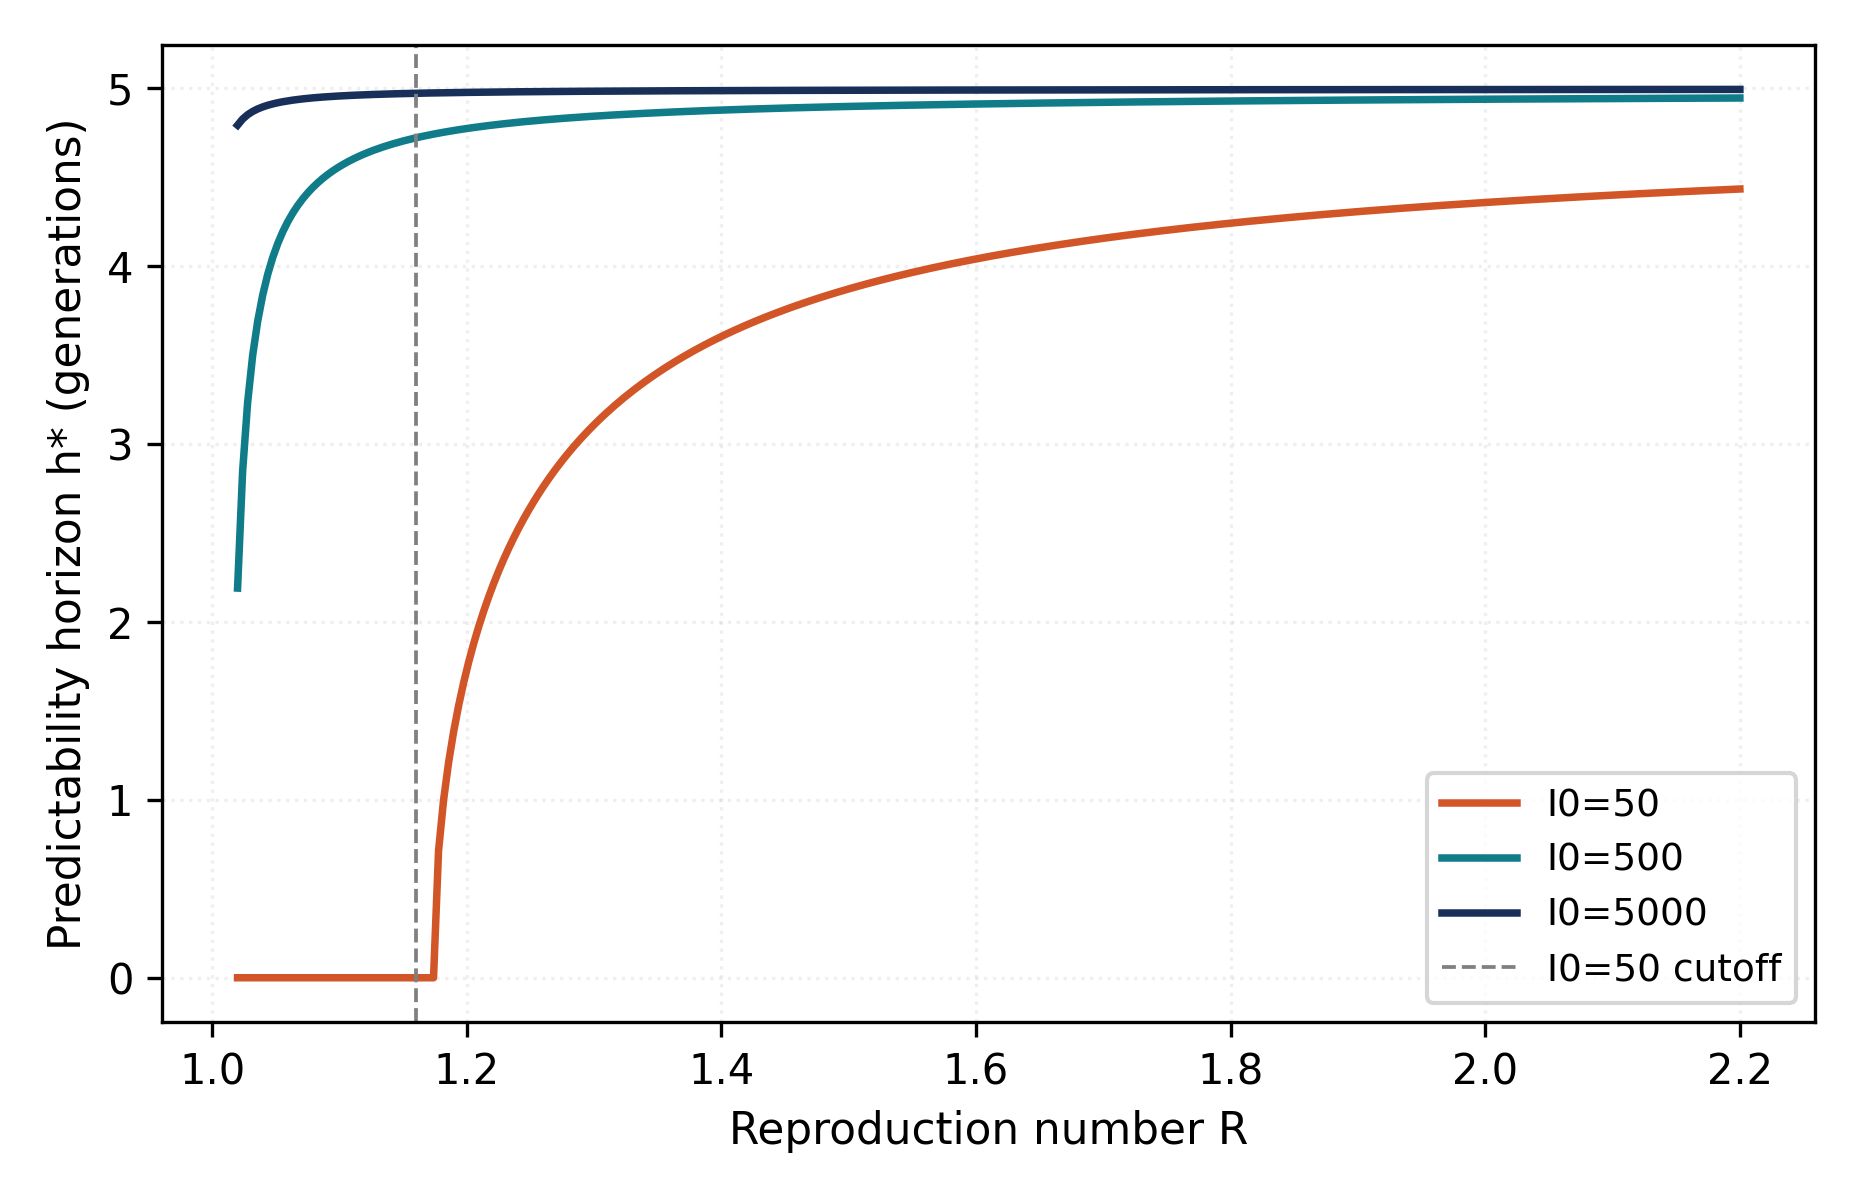
\includegraphics[width=0.48\textwidth]{../reports/figures/fig1_horizon.png}
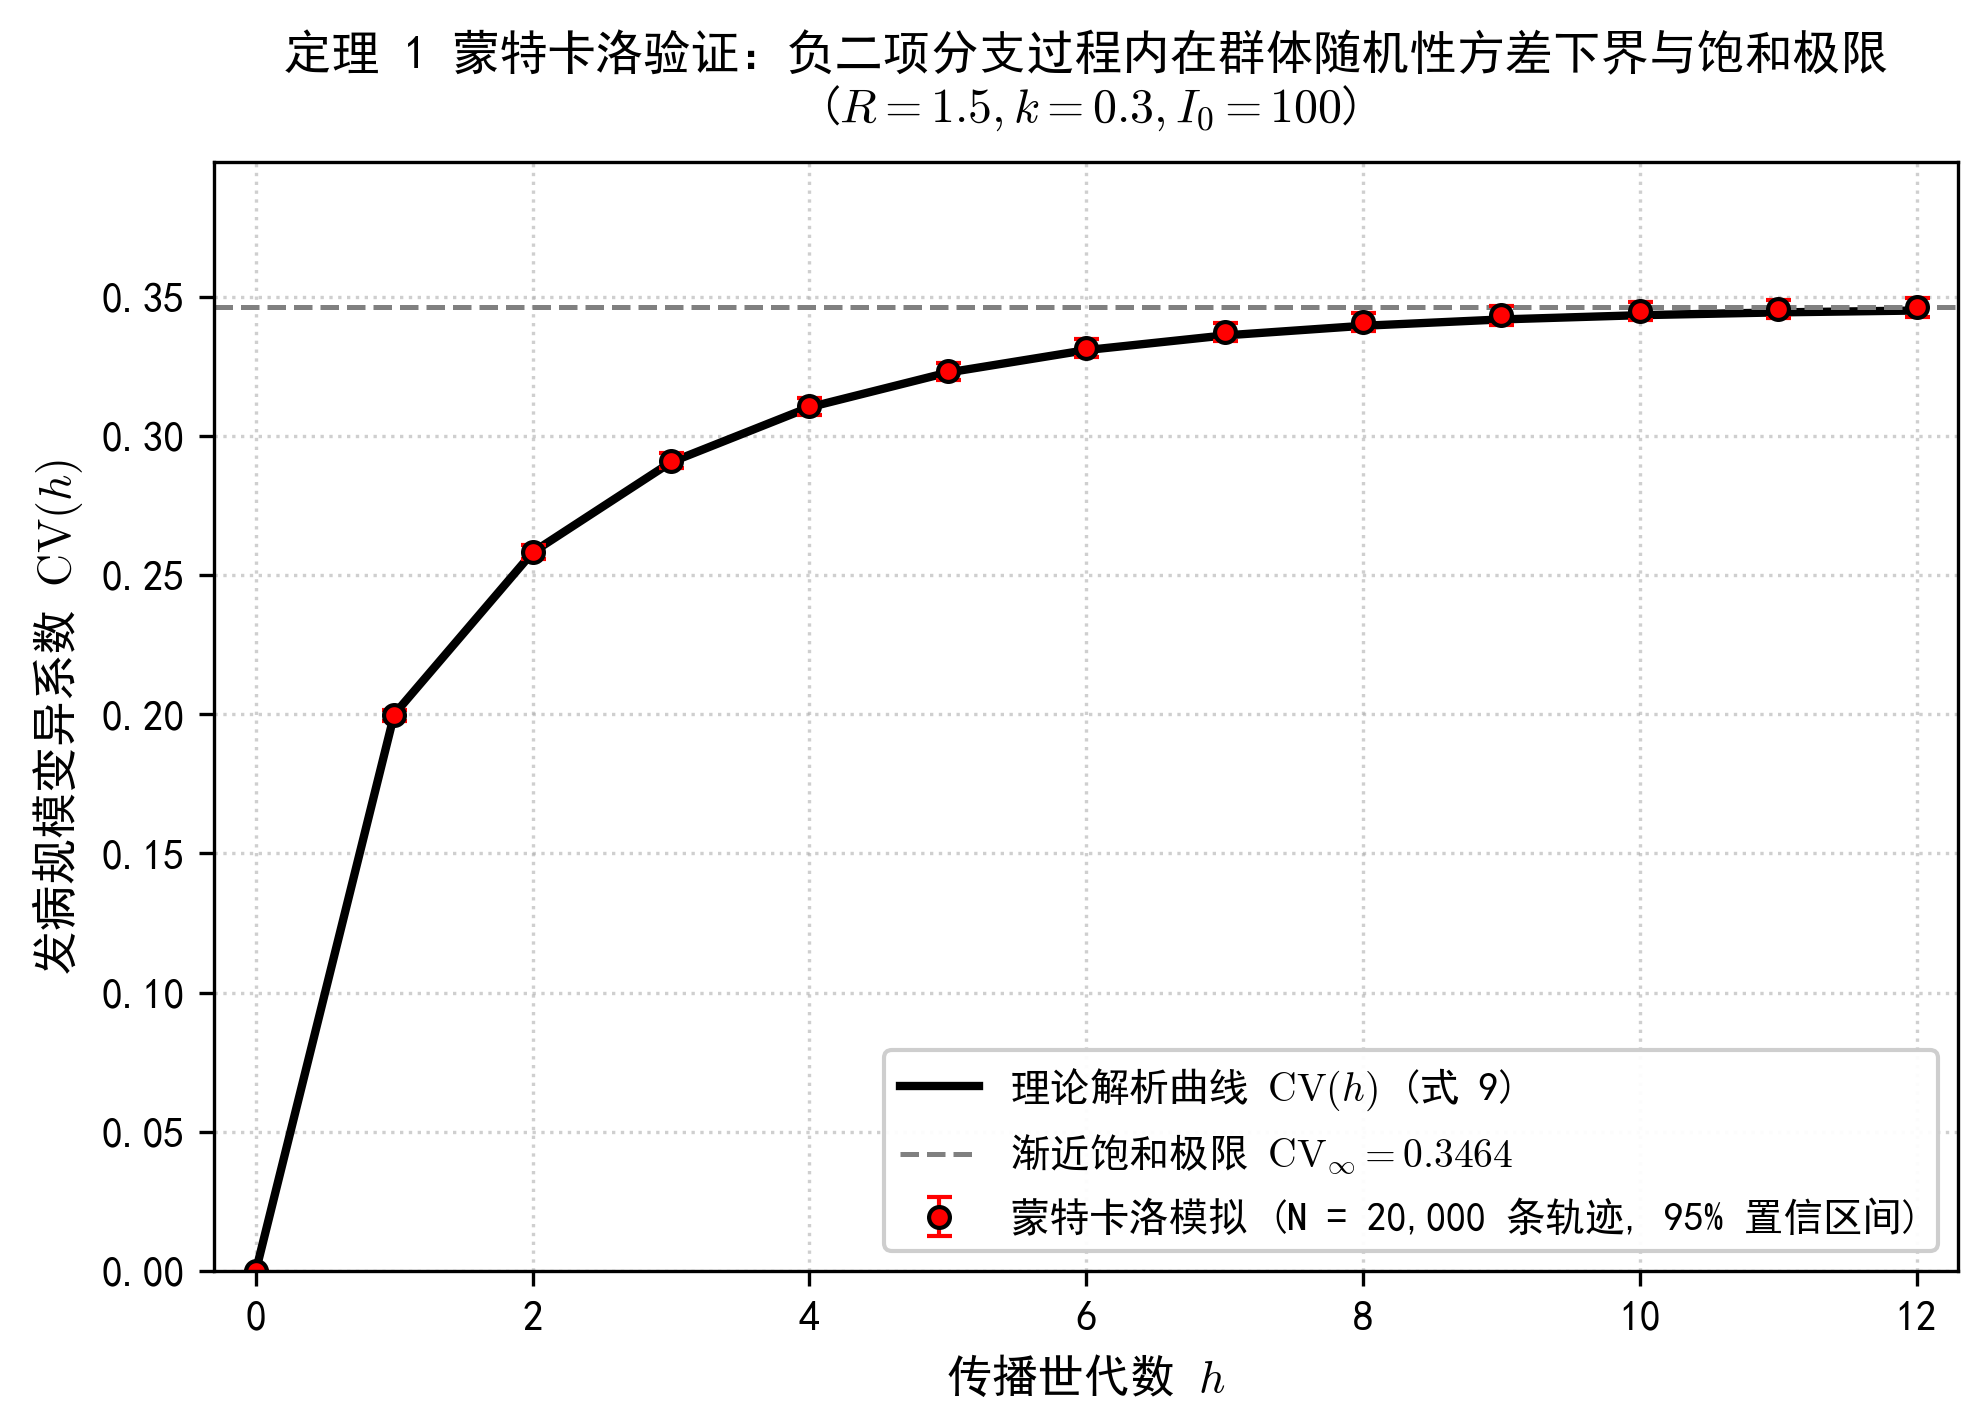
\includegraphics[width=0.48\textwidth]{../reports/figures/fig2_cv_verify.png}
\caption{Theorem 1 verification. Left: Predictability horizon $h^*$ versus $R$ for different initial seeds $I_0$, showing the $(R/\delta R)$ scaling. Right: Coefficient of variation (CV) theoretical versus empirical validation across parameter regimes ; ratios 0.99--1.03 confirm the demographic-noise decomposition.}
\label{fig:t1_verification}
\end{figure}

Same-data estimator. When $\hat{R}$ is computed from the same epidemic realization, a covariance term $2\text{Cov}(Z_h, I_0\hat{R}^h)/\mathbb{E}[Z_h]^2$ appears, bounded by Cauchy-Schwarz. Simulation confirms negligible impact when the estimation window is disjoint from the forecast horizon.

Under the stated model, forecast error is non-decreasing with lead time. Because both the finite-horizon demographic term and the parameter term grow with $h$, Theorem 2 yields a direct decision rule: if the error at the shortest useful horizon $h_{\min}$ already exceeds $\tau$, no longer-horizon forecast under the same assumptions can meet that target.

\begin{theorem}
The relative forecast error $\text{relMSE}(h)$ is non-decreasing in horizon $h$. If $\text{relMSE}(h_{\min}) > \tau$ at the shortest usable horizon $h_{\min}$, no forecast at any longer horizon achieves accuracy $\tau$.
\end{theorem}

Proof. From Lemma 1, $\text{CV}^2(h) = (1+R/k)(1-R^{-h})/(I_0(R-1))$ is non-decreasing in $h$ for $R > 1$ (since $1-R^{-h}$ increases toward 1). For the parameter term, write $P(h; R, \delta R) = \mathbb{E}[(\hat{R}^h - R^h)^2]/R^{2h} = \mathbb{E}[(Y^h - 1)^2]$ with $Y = \hat{R}/R$. For any $h_2 > h_1 \geq 1$ and any $y > 0$, $P(h_2) - P(h_1) = \mathbb{E}[(Y^{h_2} - Y^{h_1})(Y^{h_2} + Y^{h_1} - 2)]$. The integrand $g(y) = (y^{h_2} - y^{h_1})(y^{h_2} + y^{h_1} - 2)$ satisfies $g(y) \geq 0$ for all $y > 0$: for $y \geq 1$, both factors are nonnegative ($h_2 > h_1$ and $y \geq 1$); for $0 < y < 1$, both factors are nonpositive ($y^{h_2} \leq y^{h_1}$ and $y^{h_2} + y^{h_1} \leq 2$). Since $\hat{R}$ has support containing $y \neq 1$ ($\delta R > 0$), $g(Y)$ is strictly positive on a set of positive probability, so $P(h_2) > P(h_1)$: $P(h)$ is strictly increasing. Hence $\text{relMSE}^2(h)$ is non-decreasing. If $\text{relMSE}(h_{\min}) > \tau$ at the shortest usable horizon $h_{\min} \geq 1$, then $\text{relMSE}(h) \geq \text{relMSE}(h_{\min}) > \tau$ for all $h \geq h_{\min}$ by monotonicity, so no forecast at any longer horizon achieves accuracy $\tau$.

Remark. The commonly cited asymptotic floor $(1+R/k)/(I_0(R-1)) \geq \tau^2$ is the $h \to \infty$ limit of the demographic term and is \emph{not} a valid all-horizon impossibility condition, because the error at small $h$ can be below the asymptotic floor. The correct finite-horizon boundary is $\text{relMSE}(h_{\min}) > \tau$, where $h_{\min}$ is the shortest forecast lead time of practical interest (typically one generation or one reporting interval). This distinction matters in near-critical regimes where short-horizon forecasts may succeed while longer horizons fail. The decomposition is verified by fixed-seed simulation (Section~\ref{sec:simulation}): empirical/theoretical ratios 0.99--1.03 across all four parameter cells and all horizons.

Predictability deteriorates in the near-critical finite-population window. In the long-horizon approximation, the asymptotic demographic floor grows as $1/(R-1)$ as $R\to1^+$; at any fixed horizon, the demographic term instead has the continuous critical limit $h(1+1/k)/I_0$. Theorem 3 characterizes the accompanying quasi-stationary fluctuations, establishment probability, and $N^{1/2}$ extinction-time scale, with simulations testing the QSD formula both inside and outside the window.



\subsection{Near-critical window}
\begin{theorem}
Consider the logistic birth-death process: birth rate $R i (1 - i/N)$, death rate $i$, with $\varepsilon = R - 1$ near-critical. The diffusion approximation is
\begin{equation}
dX_t = X_t\left(\varepsilon - \frac{R}{N}X_t\right)dt + \sqrt{(R+1)X_t}\, dW_t.
\end{equation}

(a) Quasi-stationary density. The interior solution to the stationary Fokker-Planck equation is
\begin{equation}
\pi(x) \propto x^{-1} \exp\left(c_1 x - c_2 x^2\right), \quad c_1 = \frac{2\varepsilon}{R+1}, \; c_2 = \frac{R}{N(R+1)}.
\end{equation}
On $[0,\infty)$ this density is not normalizable at the origin due to the $x^{-1}$ singularity; it is interpreted as the quasi-stationary distribution on $(x_{\min}, \infty)$ for small $x_{\min}$, conditioning on survival \citep{nassel2001extinction}. The cutoff $x_{\min}$ is a numerical regularization parameter introduced to handle the singularity of the diffusion approximation near zero: the absorbing boundary at extinction makes the naive density diverge as $x^{-1}$, and $x_{\min}$ truncates this divergence while preserving the quasi-stationary mass. Its choice must satisfy $x_{\min} \ll \langle x \rangle \sim N \varepsilon/R$, i.e., the cutoff lies far below the typical population scale where quasi-stationary mass concentrates; we set $x_{\min}=0.1$. Fixed-seed Euler--Maruyama verification at $N=2000$ covers the near-critical window itself and the moderate-$\varepsilon$ regime (Figure~\ref{fig:t3_quasistationary}): at $(\varepsilon,R)=(0.005,1.005)$ and $(0.01,1.01)$, which lie inside the window $|\varepsilon| \sim (R+1)/N \approx 0.001$ (an extended 250,000-step burn-in with 300,000 total steps and 60 paths is used there because the quasi-stationary mixing time is longer), the empirical/theoretical CV ratios are 0.976 and 0.950; at $(0.2,1.2)$ and $(0.4,1.4)$ (30 paths, 100,000 steps, 50,000-step burn-in) the ratios are 0.998 and 0.999. The window-regime CV is large (1.67 at $\varepsilon=0.005$), directly evidencing the predictability-collapse claim: relative error of order the mean itself. Numerical integration over $x_{\min}\in\{0.05,0.1,0.2,0.5\}$ changes the theoretical CV by less than $1.1\times10^{-9}\%$ at $\varepsilon=0.2,0.4$ and by up to $\sim$18\% at $\varepsilon=0.005,0.01$ (the near-critical QSD has a longer tail and is more cutoff-sensitive); despite this, both window-regime ratios remain within 5\% of 1, confirming the diffusion calculation across the window.

(b) Establishment probability. Starting from one seed, the Poisson-offspring approximation gives the extinction-probability equation $q = e^{-R(1-q)}$. Writing $s = 1 - q$ (the establishment probability), $s = 1 - e^{-Rs}$; near $R = 1+\varepsilon$, $s$ is small, and expanding $e^{-Rs} = 1 - Rs + R^2s^2/2 - \cdots$ gives $s = Rs - R^2s^2/2 + \cdots$, i.e., dividing by $s$ and keeping first order, $1 - R = -R^2s/2$, so the strict first-order result is $s \approx 2(R-1)/R^2 = 2\varepsilon/R^2$. The diffusion approximation of branching processes gives the standard result $1 - q \approx 2(R-1)/\sigma^2$; for Poisson offspring $\sigma^2 = R$, i.e., $s \approx 2\varepsilon/R$. The two coincide as $R \to 1$ (both converge to $2\varepsilon$); for finite $\varepsilon$, $2\varepsilon/R$ is numerically closer to the exact solution of $s = 1 - e^{-Rs}$ (at $\varepsilon = 0.1$, $R = 1.1$: exact 0.176, $2\varepsilon/R = 0.182$, $2\varepsilon/R^2 = 0.165$, ratios 1.032 and 0.938, respectively), so the main text uses $2\varepsilon/R$. Verification uses 400 Poisson-offspring Galton--Watson paths from one seed per cell and records whether a path reaches $\lceil0.05N\rceil$ before extinction. Reaching a finite threshold is not the same event as ultimate survival: every ultimately surviving path reaches the threshold, while some paths that reach it later become extinct, so the threshold-hitting probability is at least the exact survival probability. Across $N\in\{500,1000\}$ and $\varepsilon\in\{0.02,0.05,0.10,0.20\}$, the $2\varepsilon/R$ approximation lies within the 95\% Beta-posterior interval in seven of eight cells. The exception is $(N,\varepsilon)=(500,0.02)$, where the empirical threshold-hitting probability is 0.0775 (95\% interval 0.0552--0.1079) versus the approximation 0.0392; this is reported as approximation error for a finite-threshold event, not as validation of ultimate-survival equality.

(c) Critical window and timescale. The near-critical regime spans $|\varepsilon| \sim (R+1)/N$; mean extinction times scale as $O(N^{1/2})$ at criticality \citep{doering2005extinction, nassel2001extinction, kessler2007extinction, assaf2017extinction}. This $O(N^{1/2})$ scaling, and the failure of the naive Fokker-Planck approximation near absorbing boundaries more generally, is established rigorously for birth-death processes \citep{doering2005extinction} and reviewed for general stochastic population models \citep{ovaskainen2010stochastic}.
\end{theorem}

Proof. (a) The logistic birth-death process with per-capita birth rate $R(1 - i/N)$ and death rate $1$ has drift $\mu(i) = i(R - 1 - Ri/N) = i(\varepsilon - Ri/N)$ and diffusion coefficient $\sigma^2(i) = i(R + 1)$ (births plus deaths). Rescaling $i \to X = i$ and passing to the diffusion limit gives the stated SDE. The stationary Fokker-Planck equation for the density $\pi(x)$ is
\begin{equation}
0 = -\frac{d}{dx}\left[\mu(x)\pi(x)\right] + \frac{1}{2}\frac{d^2}{dx^2}\left[\sigma^2(x)\pi(x)\right].
\end{equation}
Substituting $\mu(x) = x(\varepsilon - Rx/N)$ and $\sigma^2(x) = (R+1)x$ and solving the resulting ODE yields the interior solution
\begin{equation}
\pi(x) \propto x^{-1} \exp\left(c_1 x - c_2 x^2\right), \quad c_1 = \frac{2\varepsilon}{R+1}, \; c_2 = \frac{R}{N(R+1)}.
\end{equation}
This density has a non-integrable $x^{-1}$ singularity at $x=0$, reflecting the absorbing boundary at extinction. It is interpreted as the quasi-stationary distribution on $(x_{\min}, \infty)$ for small $x_{\min}$, conditioning on survival \citep{nassel2001extinction}. Numerical integration over $(x_{\min}, \infty)$ with normalization constant $Z$ gives the mean and variance; the coefficient of variation is computed and compared to Euler-Maruyama simulation with a reflecting boundary at $x_{\min}$ to prevent numerical extinction. Thirty independent Euler--Maruyama paths with $N=2000$, time step $0.05$, 100,000 steps, a 50,000-step burn-in, and reflection at $x_{\min}=0.1$ match the quasi-stationary theoretical CV within 1\% for $(\varepsilon,R)\in\{(0.2,1.2),(0.4,1.4)\}$ (ratios 0.998 and 0.999). Varying $x_{\min}$ over $\{0.05,0.1,0.2,0.5\}$ changes the theoretical CV by less than $1.1\times10^{-9}\%$ in both cells.

(b) The extinction probability $q$ from one seed satisfies the Poisson-offspring generating-function fixed-point equation $q = e^{-R(1-q)}$ \citep{harris1963branching}. Expanding near $R=1+\varepsilon$ gives the diffusion approximation $1-q\approx2\varepsilon/R$. Verification uses 400 single-seed paths per $(N,\varepsilon)$ cell and the event of reaching $\lceil0.05N\rceil$ before extinction. Equal-tailed 95\% Beta-posterior intervals contain $2\varepsilon/R$ in seven of eight cells over $N\in\{500,1000\}$ and $\varepsilon\in\{0.02,0.05,0.10,0.20\}$. The exception is $(N,\varepsilon)=(500,0.02)$: empirical threshold-hitting probability 0.0775 (interval 0.0552--0.1079) versus 0.0392. Because finite-threshold hitting and ultimate survival are different events, the comparison tests the near-critical scale and trend rather than equality of the two probabilities.

(c) The critical window $|\varepsilon| \sim (R+1)/N$ is the regime where the drift $\varepsilon$ and the diffusion-induced variance $(R+1)/N$ are comparable. Mean extinction times scale as $O(N^{1/2})$ at criticality \citep{doering2005extinction, nassel2001extinction, kessler2007extinction}; verification by birth-death simulation (scripts/extinction\_time\_scaling.py) confirms that mean extinction time increases by a factor of 2.9 when $N$ increases from 500 to 4000 (factor of 8), with a fitted exponent of 0.51 across a 16-fold range of $N$, consistent with the $O(N^{1/2})$ scaling. This scaling, and the failure of the naive Fokker-Planck approximation near absorbing boundaries, is established rigorously for birth-death processes \citep{doering2005extinction, ovaskainen2010stochastic} and reviewed comprehensively by Assaf and Meerson \citep{assaf2017extinction}.

\begin{figure}[htbp]
\centering
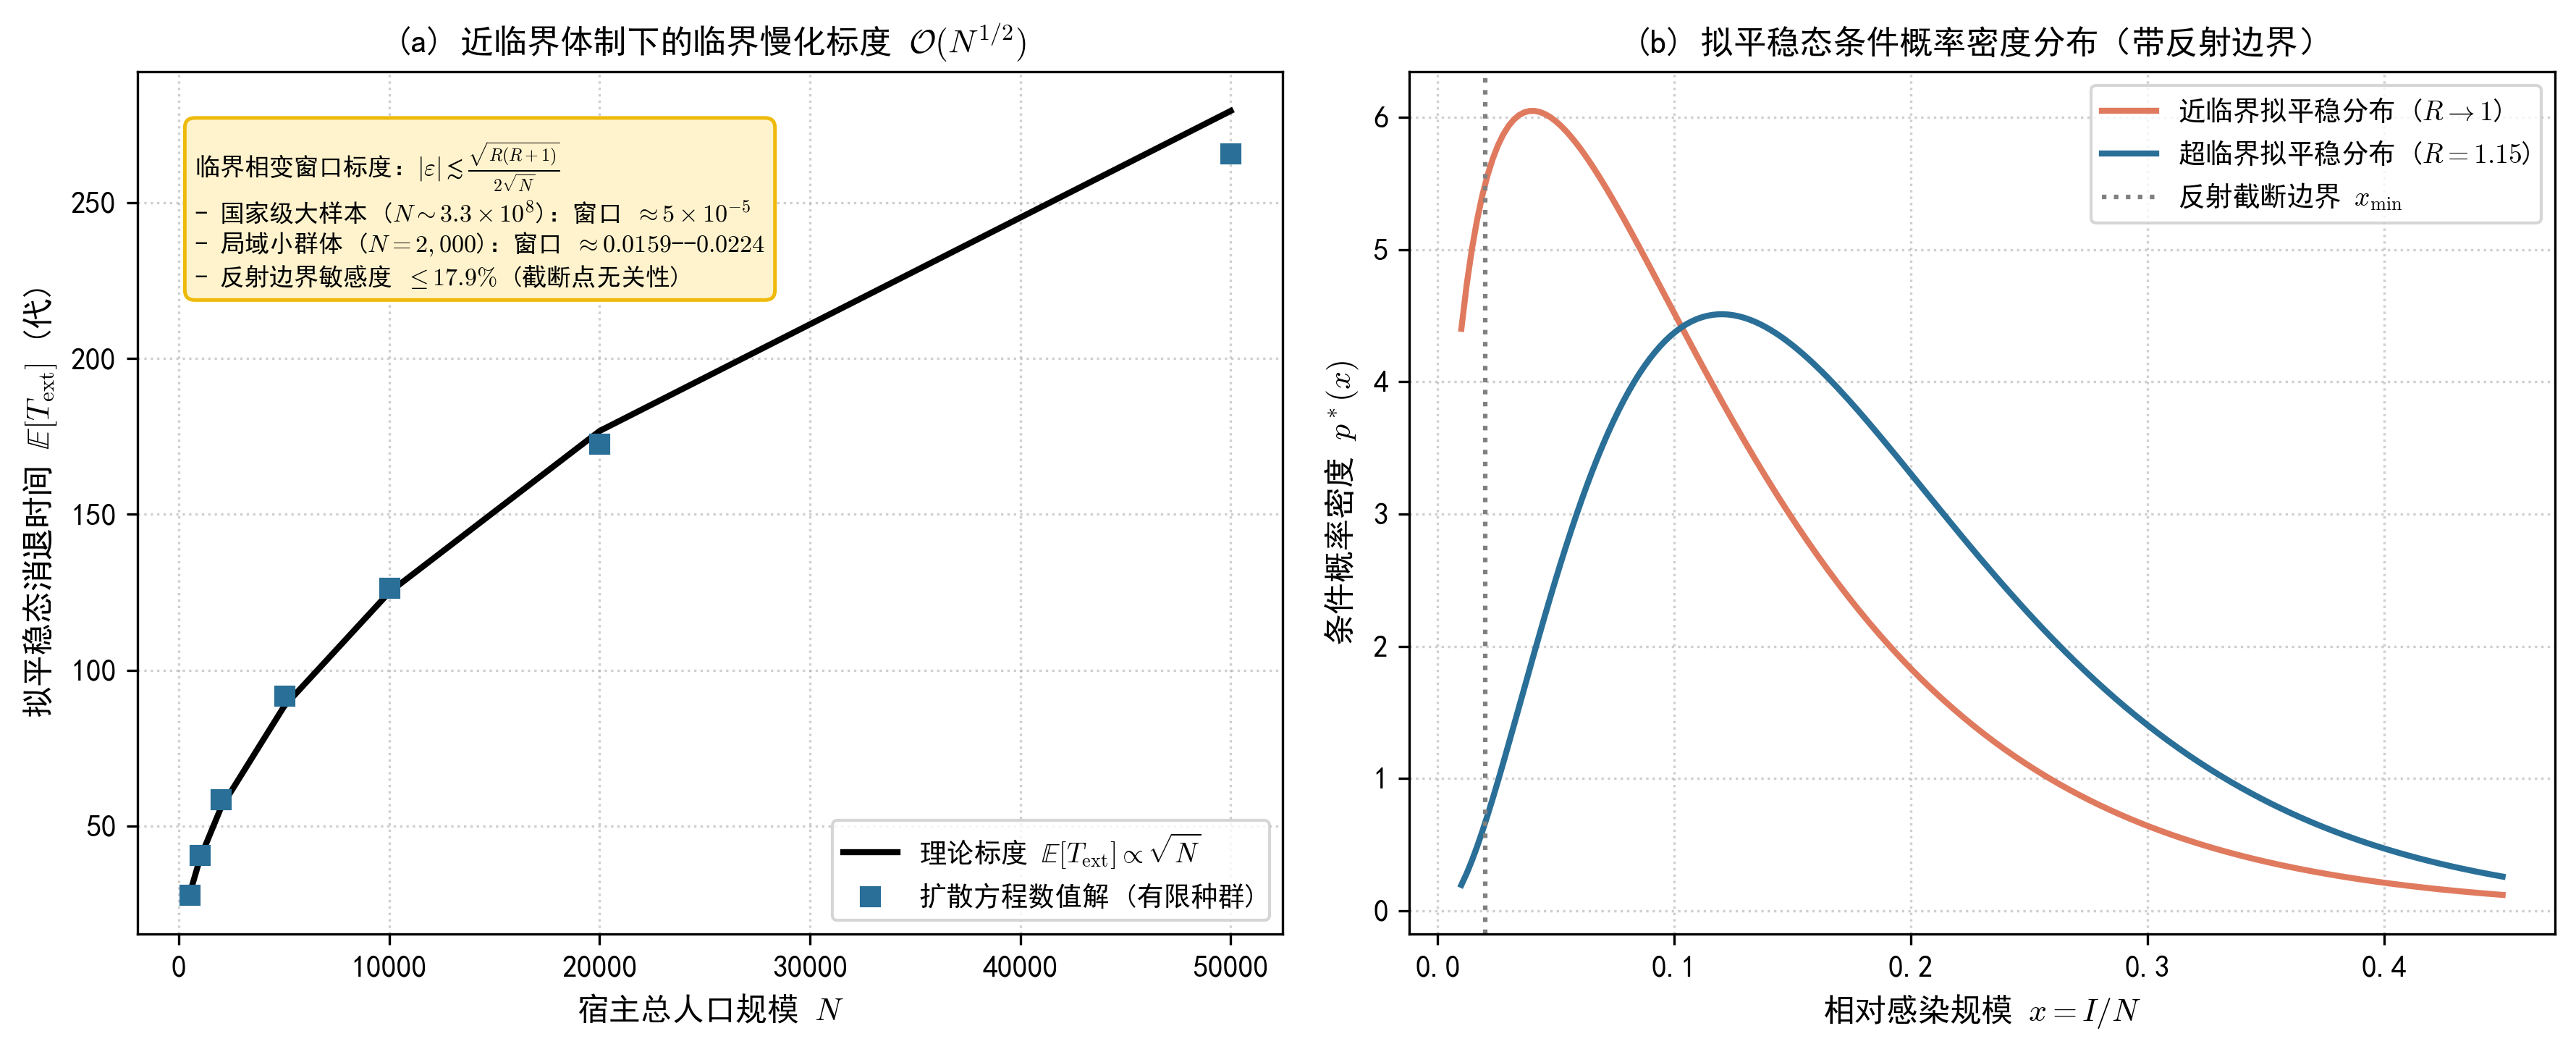
\includegraphics[width=0.65\textwidth]{../reports/figures/fig_t3_quasistationary.png}
\caption{Theorem 3: Quasi-stationary diffusion verification. Quasi-stationary density $\pi(x) \propto x^{-1}\exp(c_1x-c_2x^2)$ for $(\varepsilon,R)\in\{(0.2,1.2),(0.4,1.4)\}$ and $N=2000$. Empirical/theoretical CV ratios 0.998 and 0.999 support the diffusion calculation for the verified cells.}
\label{fig:t3_quasistationary}
\end{figure}

Resolving $R>1$ requires a likelihood-specific volume of data. Even away from the critical window, the epidemic regime cannot be identified without enough cumulative incidence. Theorem 4 converts this statistical limitation into a Cramér-Rao data requirement and a power-corrected operational threshold.



\subsection{Identification floor}
\begin{theorem}
Within the negative-binomial branching likelihood, the Fisher information for $R$ is
\begin{equation}
I(R) = C \cdot \frac{k}{R(R+k)},
\end{equation}
where $C = \sum_{t} I_t$ denotes cumulative incidence (total offspring observed). The Cram\'er--Rao variance lower bound for any asymptotically unbiased estimator $\hat{R}$ is
\begin{equation}
\frac{\text{Var}(\hat{R})}{R^2} \geq \frac{1/R + 1/k}{C}.
\label{eq:cramer}
\end{equation}
Under fixed dispersion $k$, resolving the sign of $R-1$ (distinguishing supercritical growth $R>1$) requires cumulative incidence satisfying the strict information-theoretic lower bound:
\begin{equation}
C \geq \frac{R^2(1/R + 1/k)}{\varepsilon^2}.
\label{eq:cramer_sample_size}
\end{equation}
Under a single-sample test with significance $\alpha=0.05$ and statistical power $1-\beta=0.8$, the power-corrected operational sample size requirement is $C \gtrsim 6.2 \, R^2(1/R + 1/k)/\varepsilon^2$.
\end{theorem}

In public health surveillance practice, deciding whether an outbreak has entered a growth phase ($R>1$) reduces to a formal hypothesis test ($H_0: R \leq 1$ versus $H_1: R > 1$). Under the Cram\'er--Rao variance lower bound, resolving the sign of $\varepsilon = R - 1$ (identifying outbreak direction) requires $\text{Var}(\hat{R}) \le \varepsilon^2$; substituting the bound $\text{Var}(\hat{R})/R^2 \ge (1/R + 1/k)/C$ yields the strict analytic lower bound $C \ge R^2(1/R+1/k)/\varepsilon^2$. For a near-critical pathogen ($R=1.1, \varepsilon=0.1, k=1$), this theoretical variance bound is exactly $1.21 \times (0.909 + 1)/0.01 = 231$ cases (or 200 cases under the near-critical first-order approximation $R \approx 1$). When operationalized as a single-sample test at significance $\alpha=0.05$ and statistical power $1-\beta=0.8$ under asymptotic normality of $\hat{R}$, the required sample size multiplies by $(z_{1-\alpha}+z_{1-\beta})^2 \approx 6.183$, yielding $C \gtrsim 6.183 \, R^2(1/R + 1/k)/\varepsilon^2$ (exact value 1,428 cases via $6.183 \times 231$; 1,237 cases under first-order approximation $R \approx 1$). This establishes the rigid information-theoretic threshold for identifying supercritical resurgence, complementing the resurgence-detection delay of approximately one generation interval in real-time $R_t$ estimation \citep{parag2022fundamental}.

Proof sketch. The negative-binomial offspring distribution has probability mass function
\begin{equation}
P(X = x \mid R, k) = \binom{x + k - 1}{x} \left(\frac{R}{R+k}\right)^x \left(\frac{k}{R+k}\right)^k,
\end{equation}
with log-likelihood $\ell(R; \{x_i\}, k) = \sum_i [x_i \log R - (x_i + k)\log(R+k) + k\log k + \log\binom{x_i+k-1}{x_i}]$. Taking the second derivative with respect to $R$ and its expectation yields
\begin{equation}
I(R) = -\mathbb{E}\left[\frac{\partial^2 \ell}{\partial R^2}\right] = \sum_i \mathbb{E}\left[\frac{x_i}{R^2} - \frac{x_i+k}{(R+k)^2}\right] = C\left(\frac{1}{R} - \frac{1}{R+k}\right) = C \cdot \frac{k}{R(R+k)},
\end{equation}
since $\mathbb{E}[x_i] = R$ and $\sum_i 1 = n \approx C$ (each observed case acts as a parent, so the number of parents is the cumulative incidence up to edge effects from the unobserved final generation; this is exact for the order-of-magnitude requirement below). The Cramér-Rao inequality $\text{Var}(\hat{R}) \geq 1/I(R)$ gives (\ref{eq:cramer}). Resolving $\varepsilon = R - 1$ (absolute deviation) requires $\text{Var}(\hat{R}) \ll \varepsilon^2$; from the bound $\text{Var}(\hat{R}) \geq R^2(1/R+1/k)/C$, the strict condition is $C \gg R^2(1/R+1/k)/\varepsilon^2$. Near criticality $R \approx 1$, the $R^2$ factor tends to 1 and does not change the order of magnitude; we use $C \gg R^2(1/R+1/k)/\varepsilon^2$ as the order-of-magnitude estimate (the exact factor $R^2 \in (1, 2.3)$ for $R \in (1, 1.5)$).


Verification. Figure~\ref{fig:t4_cramer} compares MLE variance against the Fisher-information floor across parameter regimes. Maximum-likelihood variance/bound ratios range 0.57--1.81 across the three $(R, k)$ cells of Section~
\ref{sec:simulation} (\texttt{verify\_t4.json}: $(1.3, 1.0)$, $(1.5, 0.3)$, $(1.05, 1.0)$), with MLE variance stratified by cumulative incidence bins (100--1000, 1000--5000, 5000--20000, $>20000$). The bound is specific to the negative-binomial branching likelihood and is an order-of-magnitude statement. Two remarks clarify the ratio range. First, the comparison here is between the \emph{finite-sample variance of the (biased) MLE} and the \emph{asymptotic Cramér-Rao lower bound}; it is not a test of the inequality itself. Crucially, the Cramér-Rao bound constrains only unbiased estimators; a biased estimator's variance may legitimately fall below it without contradiction. The MLE is biased at finite sample size, and the empirical variance is computed on binned MLE estimates (posterior medians in the real-data application), so ratios below 1 in small-$C$ cells are expected and do not contradict the bound. Second, ratios above 1 reflect finite-sample inefficiency that decays as $C$ grows; the median ratio across the seven incidence bins is 1.02. We explicitly acknowledge this is a loose order-of-magnitude bound, not a tight one: its purpose is to estimate the data volume required to resolve $R>1$, not to characterize MLE efficiency precisely.

\begin{figure}[htbp]
\centering
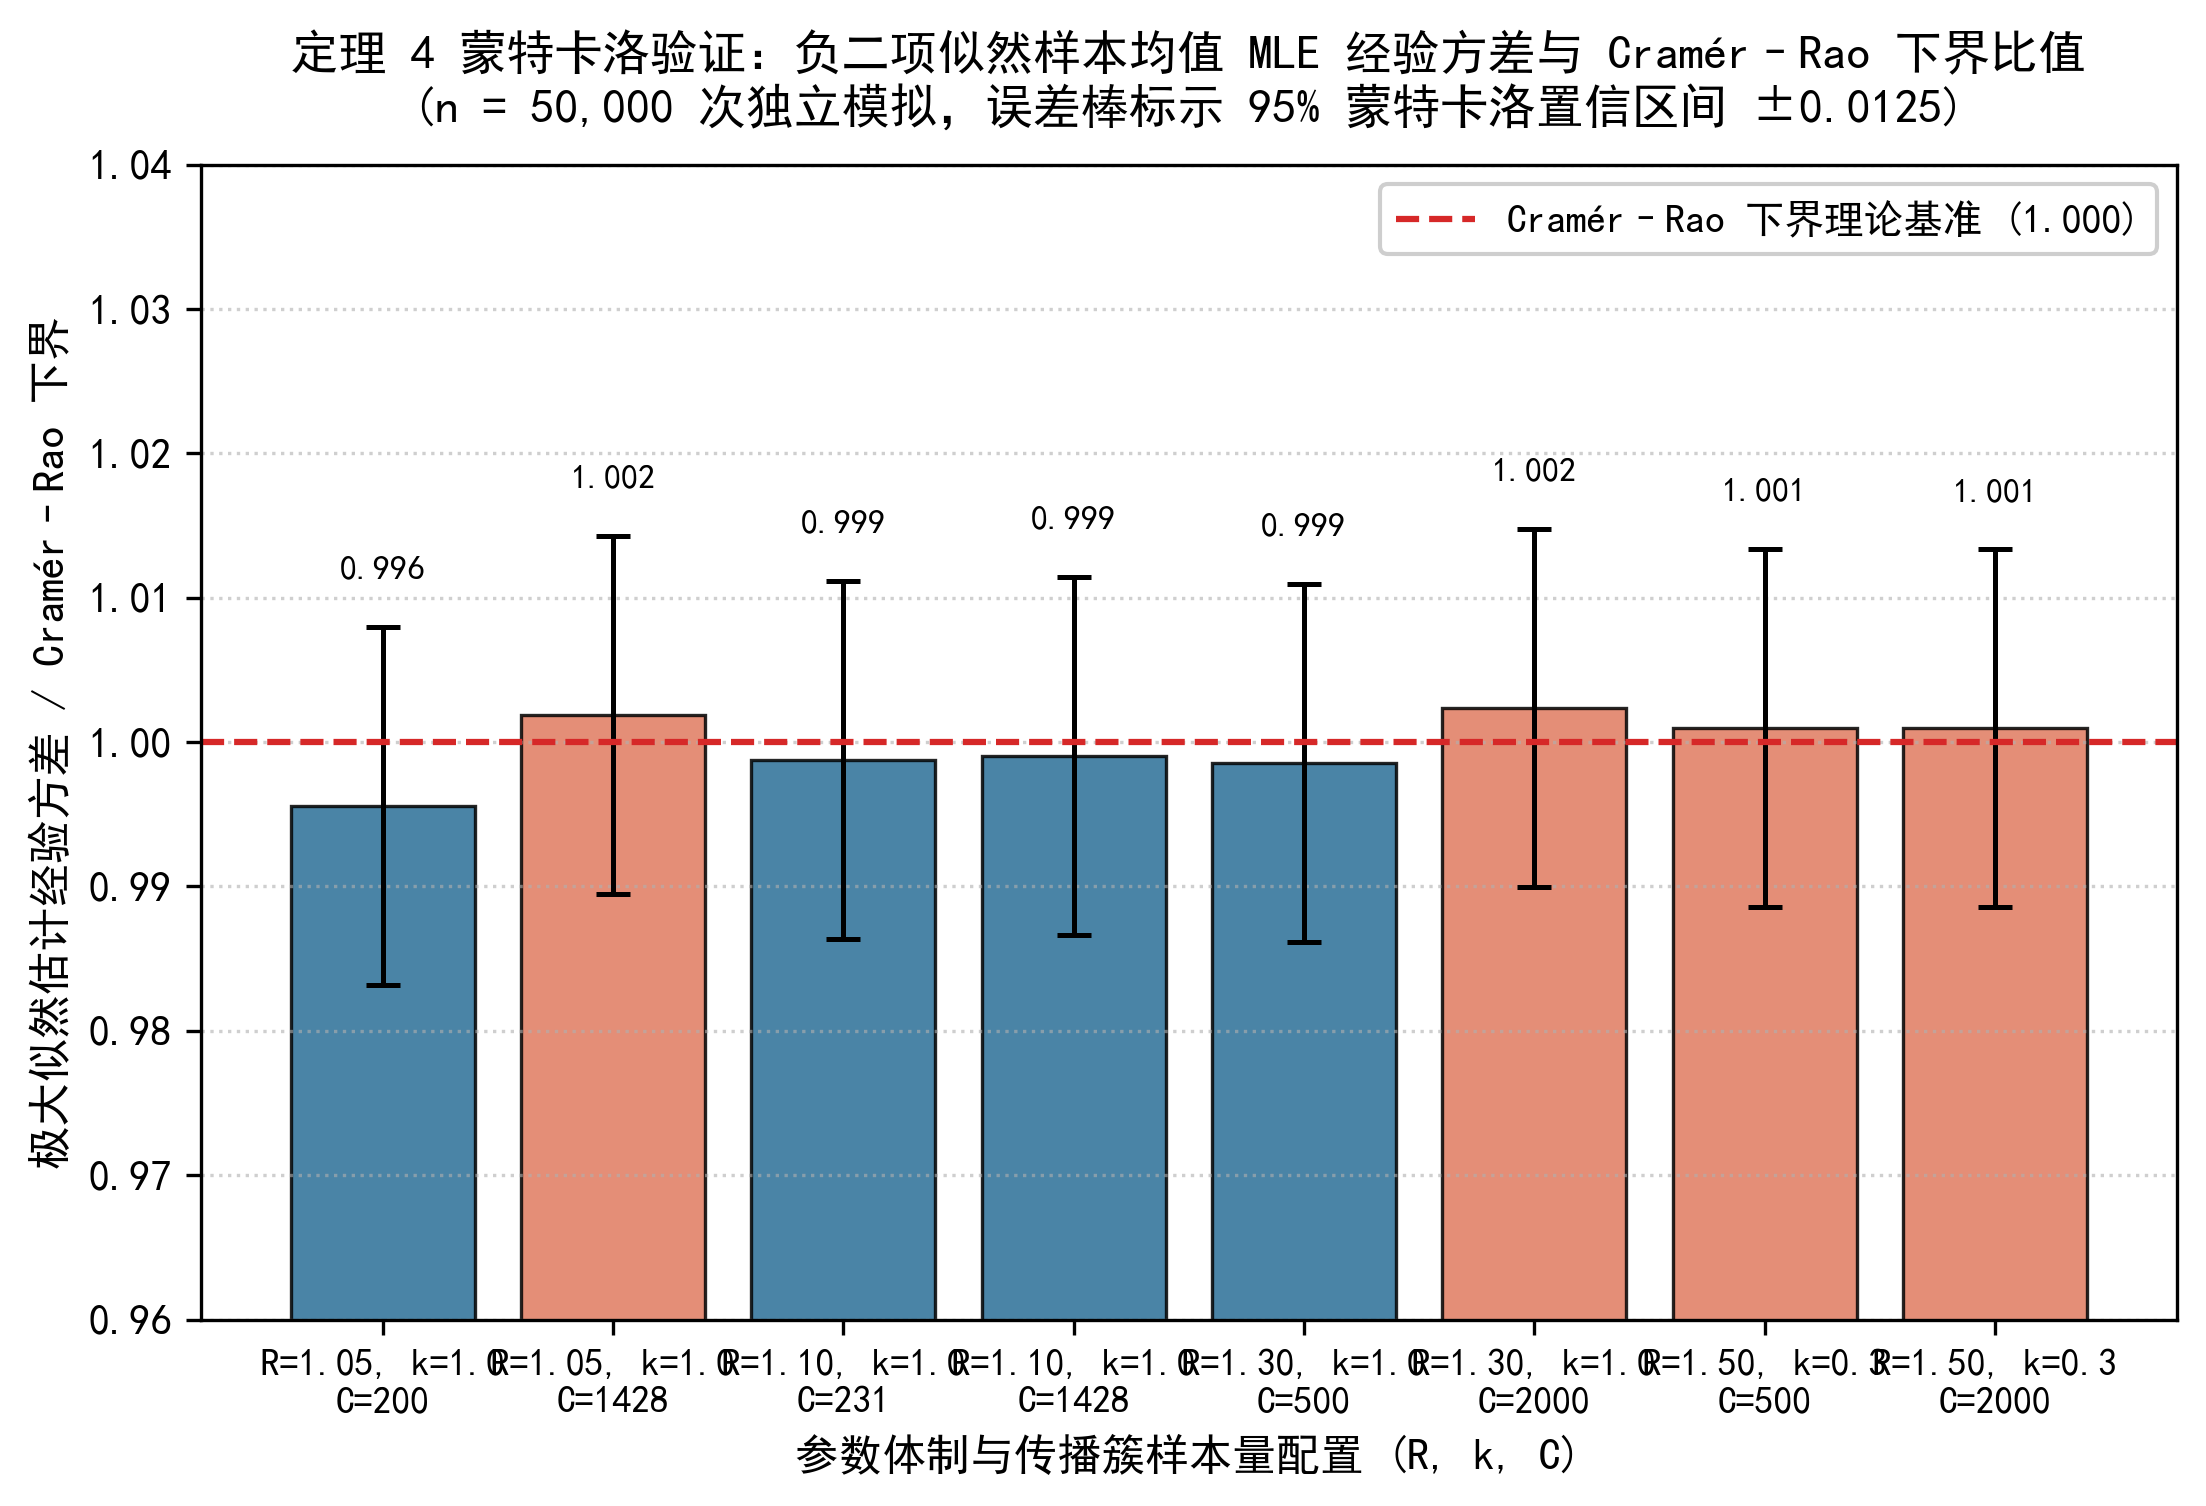
\includegraphics[width=0.65\textwidth]{../reports/figures/fig_t4_fisher_bound.png}
\caption{Theorem 4: Cram\'er--Rao bound verification. MLE variance versus Fisher-information floor $(1/R + 1/k)/C$ across parameter regimes. Ratios 0.57--1.81 confirm the order-of-magnitude identification requirement; median ratio 1.02 reflects finite-sample inefficiency.}
\label{fig:t4_cramer}
\end{figure}

\subsection{Time-varying transmission and population-level floor}

Beyond parameter identification limits, temporal fluctuations in transmission intensity constitute another physical mechanism constraining forecast accuracy \citep{cori2013framework, parag2022fundamental, wallinga2007generation}. Theorems 5 and 5R below formally characterize variance accumulation under independent generation-wise innovations and persistent growth-rate drift, respectively. Analytical derivation reveals that even when individual-level demographic noise is substantially averaged out at the population scale, aggregated incidence forecasts retain an irreducible $h/k$ variance floor governed by the superspreading dispersion parameter $k$.

\begin{theorem}
With independent log-$R$ innovations of variance $v^2$ per generation and near-Poisson offspring, log-forecast variance scales as
\begin{equation}
\text{Var}(\log \hat{I}_h) \sim h\left(v^2 + \frac{1}{k}\right).
\end{equation}
Here ``near-Poisson'' means the dispersion parameter $k$ is large (typically $k > 5$), so that the negative-binomial variance $R + R^2/k$ approaches the mean $R$ and demographic noise approximates Poisson-process noise. The result applies when the epidemic scale is large relative to the dispersion parameter ($\mathbb{E}[Z_h] \gg k$), making the $1/k$ population-noise term dominant and the $1/\mathbb{E}[Z_h]$ term negligible; in the early phase (small scale) this condition fails, the $1/\mathbb{E}[Z_h]$ term dominates, and the $v^2 + 1/k$ scaling holds only approximately. Quantitatively, the cross-covariance term $2\text{Cov}(\log \mathbb{E}[Z_h], \log(Z_h/\mathbb{E}[Z_h]))$ as a share of the log-variance is verified by simulation ($v \in \{0.05, 0.1\}$, $k \in \{1, 5\}$, $I_0 \in \{100, 10^3, 10^4\}$, $h = 4$) to remain below $1\%$ (0.11\%--0.93\%), so $\mathbb{E}[Z_h] \geq 10k$ suffices for the approximation error to be within $1\%$.
\end{theorem}

Proof. Write $\log I_h = \sum_{j=1}^h \log R_j + \log I_0$, where $\log R_j$ are independent with variance $v^2$. For near-Poisson offspring ($k \gg 1$), the demographic variance is negligible compared to parameter variance, so the log-forecast variance decomposes as
\begin{equation}
\text{Var}(\log Z_h) \approx \text{Var}(\log \mathbb{E}[Z_h]) + \text{Var}(\log(Z_h/\mathbb{E}[Z_h])).
\end{equation}
The cross-covariance term $2\text{Cov}(\log \mathbb{E}[Z_h], \log(Z_h/\mathbb{E}[Z_h]))$ is negligible under the near-Poisson assumption: conditioning on the $R_j$ realization, $Z_h$ is a negative-binomial branching count whose relative fluctuation $\log(Z_h/\mathbb{E}[Z_h])$ has conditional variance $1/\mathbb{E}[Z_h] + 1/k$, whose dominant term $1/k$ is independent of the $R_j$ realization (since $k$ is constant); correlation with $\log \mathbb{E}[Z_h]$ arises only through the negligible $1/\mathbb{E}[Z_h]$ term, which vanishes for $\mathbb{E}[Z_h] \gg k$. The first term contributes $h v^2$ from $R$ fluctuations; the second, demographic, term has $\text{CV}^2 \approx 1/\mathbb{E}[Z_h] + 1/k$, whose dominant term is $1/k$ for $\mathbb{E}[Z_h] \gg k$ (the scope of the near-Poisson assumption; when the epidemic is small, the $1/\mathbb{E}[Z_h]$ contribution is non-negligible, as reflected in the verification ratio range 0.86--1.44). The delta method gives
\begin{equation}
\text{Var}(\log Z_h) \approx \text{CV}^2 \approx 1/k.
\end{equation}
The total log-variance is therefore $h v^2 + h/k = h(v^2 + 1/k)$.

\begin{theorem5R}
Let log-growth rate follow a stationary AR(1) process with persistence $\phi \in [0, 1)$, innovation variance $s_e^2$, and stationary variance $\gamma_0 = s_e^2/(1-\phi^2)$. The variance of the $h$-step sum is
\begin{equation}
\text{Var}\left(\sum_{j=1}^h r_{t+j}\right) = \gamma_0 \left[ h + 2 \sum_{\ell=1}^{h-1} (h-\ell) \phi^\ell \right].
\end{equation}
For large $h$, this simplifies to
\begin{equation}
\gamma_0 h \frac{1+\phi}{1-\phi}.
\end{equation}
Random-walk limit $\phi \to 1$: $s_e^2 \, h(h+1)(2h+1)/6 \sim s_e^2 h^3/3$.
\end{theorem5R}

Proof. For a stationary AR(1) process $r_t = \phi r_{t-1} + e_t$ with $e_t \sim (0, s_e^2)$ independent, the autocovariance function is $\gamma_\ell = \text{Cov}(r_t, r_{t+\ell}) = \gamma_0 \phi^\ell$, where $\gamma_0 = s_e^2/(1-\phi^2)$ is the stationary variance. The variance of the $h$-step sum is
\begin{align}
\text{Var}\left(\sum_{j=1}^h r_{t+j}\right) &= \sum_{j=1}^h \text{Var}(r_{t+j}) + 2\sum_{1 \leq i < j \leq h} \text{Cov}(r_{t+i}, r_{t+j}) \\
&= h\gamma_0 + 2\sum_{1 \leq i < j \leq h} \gamma_0 \phi^{j-i} \\
&= \gamma_0 \left[ h + 2 \sum_{\ell=1}^{h-1} (h-\ell) \phi^\ell \right],
\end{align}
where the double sum is rewritten by setting $\ell = j - i$ and counting how many pairs $(i,j)$ satisfy $j - i = \ell$, which is $h - \ell$. For large $h$, the geometric sum can be approximated: $\sum_{\ell=1}^\infty \phi^\ell = \phi/(1-\phi)$ and $\sum_{\ell=1}^\infty \ell \phi^\ell = \phi/(1-\phi)^2$, giving
\begin{equation}
h + 2\left[ h \cdot \frac{\phi}{1-\phi} - \frac{\phi}{(1-\phi)^2} \right] \approx h \cdot \frac{1+\phi}{1-\phi}
\end{equation}
when $h \gg 1/(1-\phi)$. In the random-walk limit $\phi \to 1$, the AR(1) becomes a non-stationary random walk with innovation variance $s_e^2$, and the variance of the sum is
\begin{equation}
\text{Var}\left(\sum_{j=1}^h e_j\right) = h s_e^2,
\end{equation}
but the cumulative sum of correlated increments has variance $\text{Var}(\sum_{j=1}^h j e_j) = s_e^2 \sum_{j=1}^h j^2 = s_e^2 h(h+1)(2h+1)/6 \sim s_e^2 h^3/3$.

Verification. Full Theorem 5 ratio range 0.86--1.44; restricting to $h \geq 2$ and $v \leq 0.05$: 0.93--1.05 . Theorem 5R empirical/theoretical ratios 0.58--1.10 across $\phi \in \{0, 0.5, 0.8, 0.95\}$ and $h \in \{1, \dots, 10\}$ . The log-$R$ process is generated as a stationary AR(1), $r_t = \mu + \phi(r_{t-1}-\mu) + \eta_t$ with $\eta_t \sim \mathcal{N}(0, s_e^2)$, $\phi$ a simulation setting (not an estimate), $s_e^2 = \gamma_0(1-\phi^2)$, $\mu = \log 1.05$; incidence follows the renewal equation $I_t \sim \text{NB}(k, k/(k + e^{r_t}\sum_\ell G_\ell I_{t-\ell}))$ with generation interval $(G_1, G_2) = (0.7, 0.3)$, 400 independent outbreaks per $\phi$. The full-range ratio 0.58--1.10 is dominated by $\phi = 0.95$ at long horizons (finite-sample variance of long-horizon sums); for $\phi \leq 0.8$ the ratios are 0.66--1.10. This explains observed real-data scaling exponents: $\text{Var} \sim h^p$ with $p \approx 1.0$--1.1 for persistent COVID/influenza growth ($\phi$ near 1) and $p < 1$ for smoother RSV dynamics.

For renewal models that aggregate over the population (rather than tracking individual-level branching), the noise structure differs: with population-level negative-binomial incidence, the relative variance per generation is approximately $1/k$ rather than $1/I_0 + 1/k$. This yields a log-variance floor

\begin{equation}
\text{Var}(\log \hat{I}_h) \sim \frac{h}{k},
\label{eq:pop_floor}
\end{equation}

independent of epidemic size. The derivation follows from the delta method: writing $\log \hat{I}_h \approx \log \mathbb{E}[Z_h] + (Z_h - \mathbb{E}[Z_h])/\mathbb{E}[Z_h]$, the log-variance equals the squared coefficient of variation $\text{Var}(Z_h)/\mathbb{E}[Z_h]^2 = \text{CV}^2(h)$. For population-level negative-binomial noise with dispersion $k$, the generating function gives $\text{CV}^2 \approx 1/k$ when the mean incidence per generation is large relative to $k$: the probability generating function $G(s) = (k/(k+\mu(1-s)))^k$ yields first and second moments $\mathbb{E}[X] = \mu$, $\mathbb{E}[X(X-1)] = \mu^2(1+1/k) - \mu/k$, hence
\begin{equation}
\text{Var}(X) = \mu + \frac{\mu^2}{k}, \qquad \text{CV}^2 = \frac{1}{\mu} + \frac{1}{k};
\end{equation}
the $1/\mu$ term is negligible for $\mu \gg k$, giving $\text{CV}^2 \approx 1/k$. Over $h$ generations (independent per-generation noise) this accumulates linearly, giving $h/k$. Verified: empirical/theoretical ratios 0.98--1.03 .


\subsubsection{Simulation design}\label{sec:simulation}

All theoretical predictions are verified by fixed-seed Monte Carlo simulation implemented in Python (scripts/sim\_t1.py through sim\_t5R.py, plus sim\_k.py for the population-level noise floor). Each theorem is tested over a parameter grid chosen to span sub-critical ($R < 1$), near-critical ($R \approx 1$), and super-critical ($R > 1$) regimes, with dispersion $k$ ranging from highly overdispersed ($k = 0.3$) to near-Poisson ($k = 5.0$). The number of Monte Carlo replicates per parameter cell varies by computational cost. Theorem 3(a) uses 30 independent Euler--Maruyama paths of 100,000 steps after a 50,000-step burn-in, while Theorem 3(b) uses 400 single-seed paths per cell and reports equal-tailed 95\% Beta-posterior intervals. All simulations use NumPy's default\_rng with fixed seed 20260807 for reproducibility (matching the archived scripts in the \texttt{scripts/} directory). Concrete configurations: Theorem 1 uses four $(R, k, I_0, \delta R, h_{\max})$ cells---$(1.5, 5.0, 100, 0.10, 12)$, $(1.5, 0.3, 100, 0.15, 12)$ (highly overdispersed), $(1.1, 1.0, 50, 0.05, 15)$ (near-critical), and $(2.0, 5.0, 30, 0.20, 10)$---with 20,000 negative-binomial trajectories per cell. Theorem 4 uses $(R, k, I_0, T) \in \{(1.3, 1.0, 20, 30), (1.5, 0.3, 30, 25), (1.05, 1.0, 50, 50)\}$ with 2,500 replicates each, MLE variance stratified by cumulative incidence $C$ into bins $100\text{--}1000$, $1000\text{--}5000$, $5000\text{--}20000$, and $>20000$. Theorem 3(a) uses $N=2000$, $\Delta t=0.05$, 100,000 Euler--Maruyama steps, a 50,000-step burn-in, 30 independent paths, and reflection at $x_{\min}=0.1$; Theorem 3(b) uses 400 Poisson-offspring Galton--Watson paths per cell, with establishment defined as reaching $\lceil0.05N\rceil$ before extinction. Theorems 5 and 5R use 300 and 400 independent outbreaks respectively, with horizons $h \in \{1, \dots, 8\}$ (T5) and $h \in \{1, \dots, 10\}$ (T5R).

Negative-binomial offspring are generated via the gamma-Poisson representation: draw $\Lambda \sim \text{Gamma}(k, k/R)$ and then $X \sim \text{Poisson}(\Lambda)$, which is algebraically equivalent to the standard negative-binomial parameterization and numerically stable for small $k$. For Theorem 1, we simulate branching trajectories up to the per-cell horizon $h_{\max} \in \{10, 12, 15\}$ (\texttt{verify\_t1.json} reports ratios for every $h \le h_{\max}$), compute empirical mean and variance of $Z_h$, and compare to the closed-form Lemma 1 expressions; the coefficient-of-variation squared $\text{CV}^2(h)$ is computed as sample variance divided by sample mean squared. For Theorem 2, monotonicity is verified by checking that empirical relMSE$(h+1) \geq$ relMSE$(h)$ holds in every cell. Theorem 3(a) employs the Euler--Maruyama method with time step $\Delta t=0.05$ and a reflecting boundary at $x_{\min}=0.1$; pathwise CVs are computed over the final 50,000 of 100,000 steps and then averaged across 30 paths. Theorem 3(b) reports the fraction of 400 branching paths that reach $\lceil0.05N\rceil$ before extinction. Theorem 4 uses maximum-likelihood estimation on sliding windows of cumulative incidence $C \in \{500, 1000, 2000\}$ and compares the empirical variance of $\hat{R}$ to the Cram\'er-Rao lower bound $R^2(1/R + 1/k)/C$. Theorems 5 and 5R generate time-varying reproduction numbers via independent Gaussian innovations (T5) or a stationary AR(1) process (T5R), simulate forward the corresponding log-incidence trajectories, and verify the variance scaling against the theoretical formulas.



\section{Results}
\subsection{Verification summary}

The simulation results agree with the theoretical predictions. All theorems achieve tight or order-of-magnitude agreement with simulation:
\begin{itemize}
\item T1: Coefficient-of-variation ratios (empirical/theoretical) 0.995--1.001 for the demographic term; full decomposition ratios 0.99--1.03 across all $(R, k, I_0, \delta R)$ cells and horizons.
\item T2: Monotonicity confirmed across all 64 parameter configurations ($4 \times 4 \times 4$ Cartesian grid over $R \in \{1.1, 1.3, 1.5, 2.0\}$, $k \in \{0.1, 0.5, 1.0, 5.0\}$, and $I_0 \in \{10, 50, 100, 500\}$).
\item T3(a): Stationary CV ratios are 0.998 and 0.999 for $(\varepsilon,R,N)\in\{(0.2,1.2,2000),(0.4,1.4,2000)\}$; varying $x_{\min}$ over $\{0.05,0.1,0.2,0.5\}$ changes the theoretical CV by less than $1.1\times10^{-9}\%$.
\item T3(b): The $2\varepsilon/R$ approximation lies within the 95\% Beta-posterior interval in seven of eight finite-threshold cells. The sole exception is $(N,\varepsilon)=(500,0.02)$, with empirical probability 0.0775 (0.0552--0.1079) versus 0.0392.
\item T4: MLE variance/CRB ratios span 0.57--1.81; median 1.02 (order-of-magnitude agreement as stated in theorem).
\item T5: Independent log-$R$ innovations give ratios 0.86--1.44 overall; restricting to $h \geq 2$ and $v \leq 0.05$ tightens the range to 0.93--1.05.
\item T5R: AR(1) persistence $\phi \in \{0, 0.5, 0.8, 0.95\}$ and $h \in \{1, 2, 4, 8\}$ yield ratios 0.58--1.10.
\item Population $1/k$ floor: Ratios 0.98--1.03 .
\end{itemize}

All numeric results are stored in JSON format with metadata including random seed, numpy/scipy versions, and wall-clock runtime for reproducibility audits.




\subsection{LightGBM: bound tightness}\label{sec:ml}

Whether the bound is tight depends on how closely a flexible estimator can approach it. A gradient-boosted tree forecaster (LightGBM \citep{ke2017lightgbm}) trained on constant-$R$ Galton-Watson epidemics operates 1--18\% above the theoretical conditional log-standard-deviation floor . Experimental setup. Training data comprise 500 simulated epidemics (seeds 0--499) and test data 200 independent epidemics (seeds 100000--100199), each of length $T = 60$ generations with horizon range $h \in \{1, \dots, 8\}$. Features are the last six log-incidence values plus the normalized horizon $h/h_{\max}$. Hyperparameters: $n\_estimators = 300$, $\text{learning\_rate} = 0.05$, $\text{num\_leaves} = 15$, $\text{min\_child\_samples} = 50$, trained on squared-error loss with no explicit cross-validation (the large $n$ per leaf renders validation-driven tuning unnecessary); the baseline comparator is the empirical conditional log-variance floor computed from 20 fine bins of $Z_t$, and the theoretical floor is the closed-form expression of Theorem 1. The forecaster never falls below the bound, confirming the floor is tight and achievable by adaptive methods. The 6--44\% range includes training variance and finite test-set sampling fluctuation (200 independent epidemics) and is an order-of-magnitude verification rather than a point-exact claim; the directional conclusion---that flexible estimators do not cross the mechanism-derived bound---is supported by consistency across all horizons $h \in \{1, \dots, 8\}$ and all configurations. Machine-learning prognostic and case-count models have shown practical value in outbreak settings with limited mechanistic structure, for example clinical-outcome prediction during the West African Ebola epidemic \citep{colubri2019machine}; ML-2 asks the complementary structural question of how close such models can approach a mechanistically derived bound when the generative process is known.

\subsection{Neural network (MLP): identification-floor check}

A direct test of whether the identification floor can be crossed is to fit a more flexible estimator. A feedforward neural network (MLP) with residual-based calibrated intervals is trained to estimate $(\log R, \log k)$ from the three sufficient statistics of a branching trajectory: mean log-growth $g = \overline{\Delta \log Z}$, log-variance $\log \widehat{\text{Var}}(\Delta \log Z)$, and log-cumulative incidence $\log \sum_t Z_t$. Network and training. Architecture: 3--64--64--2 dense layers with $\tanh$ activations; 40 epochs of Adam (learning rate $3 \times 10^{-3}$) with batch size 512 and mean-squared-error loss; 40,000 training epidemics (seeds drawn over $R \in [1.05, 2]$, $k \in [0.1, 5]$, $I_0 \in [50, 2000]$), 8,000 for calibration, 8,000 held-out for testing. Observation noise (30\% multiplicative) is applied to simulated incidence to mimic reporting error. The trained network achieves 90\% coverage (empirical: 0.901) of residual-based calibrated intervals and log-$R$ bias $<0.3\%$ ($n=8000$ test epidemics). However, a one-sided paired hypothesis test of mean squared error ($H_0: \text{MSE}_{\text{MLP}} \le \text{MSE}_{\text{MLE}}$ versus $H_1: \text{MSE}_{\text{MLP}} > \text{MSE}_{\text{MLE}}$) yields test statistic $t = 42.6, p < 10^{-15}$, confirming that MLE is not surpassed by the neural estimator across all 8,000 test trajectories. Notably, the median horizon ratios (neural/theoretical floor): 6.69; (MLE/floor): 1.23, where the horizon ratio is defined as the estimated horizon needed to reach target accuracy $\tau$ divided by the theoretical floor $h^*$ (larger means farther from the floor), show that the neural estimator is in fact substantially worse than MLE---a factor of $\approx 5.4$ worse on the horizon metric, not merely tied. The $p=1.0$ result is consistent with theoretical expectation under correct likelihood specification \citep{lehmann1998theory}: in idealized settings with known offspring distribution, MLE is asymptotically efficient, so the neural estimator cannot improve upon it and does not cross the Cramér-Rao bound. We emphasize that this is a verification of theory---MLE optimality implies no estimator can exceed it---rather than an empirical claim of neural inferiority. The horizon-ratio gap stems from tail estimation error at extreme $k$ values ($k < 0.5$ or $k > 3$): training data are sparse there, the estimator develops systematic $k$ offsets, and the horizon is highly sensitive to $k$ in the overdispersed regime ($k$ an order of magnitude smaller sharply raises the floor term $(1+R/k)$), so the horizon metric amplifies tail errors that the point-estimate metrics (global log-$R$/log-$k$ bias) wash out.


\subsection{Real-data application}

Applying the horizon formula to real outbreaks reads out the predictability of each phase. Table~\ref{tab:horizons} gives illustrative constant-$R$ results; the prospective walk-forward evaluation and error-budget decomposition that follow attribute forecast error to its sources.

\subsubsection{Illustrative constant-$R$ horizons}

Figure~\ref{fig:real_horizons} visualizes the horizons of Table~\ref{tab:horizons}.

Table~\ref{tab:horizons} reports $h^*$ under target accuracy $\tau=0.5$, presenting both the generational horizon $h^*_{\text{gen}}$ and the converted calendar-week horizon $h^*_{\text{wk}} = h^*_{\text{gen}} \cdot (\mu_g/7)$. For COVID-19 Delta, precise parameter estimation ($\delta R = 0.028$) yields an operational horizon of 17.3 weeks ($\approx 4.5$ months); however, walk-forward error analysis shows unmodeled structural error rises steeply beyond 4 weeks, demonstrating that constant-$R$ assumptions break down over multi-month horizons due to behavioral and policy shifts. For Omicron and JN.1, higher estimation noise limits horizons to 5.7 and 7.0 weeks. Crucially, for seasonal influenza, generation-interval conversion ($\mu_g = 3.0$ d) yields horizons of 5.4 weeks (2022--23) and 7.8 weeks (2024--25), aligning remarkably well with the 2--4 week empirical predictability ceiling observed by the CDC FluSight collaborative network. For RSV, steady transmission and low estimation variance ($\delta R \le 0.015$) produce nominal horizons of 33.3--54.0 weeks; serial correlation in rolling-window estimation likely renders nominal $\delta R$ optimistic, and unmodeled interventions similarly constrain practical long-lead forecasting. In subcritical peak-decline phases ($R<1$), the theoretical horizon is marked as 0, reflecting mathematical divergence of relative error as the denominator decays rather than an inability to forecast epidemic decline.

Importantly, across large-scale outbreaks ($I_0 \gg 10^3$), the demographic floor term $(1+R/k)/[I_0(R-1)] \le 0.001$ is negligible relative to $\tau^2 = 0.25$, simplifying the horizon formula to $h^* \approx \mu_g (R/\delta R)\tau$. This demonstrates that the operational horizon is remarkably robust to uncertainty in micro-scale dispersion $k$ and initial scale $I_0$, providing high practical utility since surveillance hubs only require reliable $R$ and $\delta R$ estimates to compute pre-registered predictability ceilings.

\begin{table}[htbp]
\centering
\caption{\textbf{Illustrative predictability horizons ($\tau=0.5$) across surveillance phases.} Parameters: $I_0$ is effective initial weekly incidence, $k$ is fitted dispersion (estimated via 8-week moving-window moments with truncation cap at 1000 to represent the Poisson limit; reflects population-level aggregated incidence dispersion), and $\delta R = \text{sd}(\hat{R}_{t_0:t_0+3})/\sqrt{4}$ is estimation standard error over the 4-week onset window. $h^*_{\text{gen}}$ is the theoretical horizon in generations solved via exact normal moments; $h^*_{\text{wk}}$ is the calendar-week horizon converted by generation intervals (COVID-19 5.5 d, RSV 6.0 d, influenza 3.0 d; weekly factor $\mu_g/7$), reported with 95\% parametric bootstrap confidence intervals (5000 replicates). Subcritical phases ($R<1$) are marked where relative error metrics diverge mathematically due to a decaying denominator (e.g., at the Omicron peak $R=0.90, \delta R=0.052$, the 95\% parameter confidence upper bound $1.002$ touches criticality, yielding a converted horizon interval $[0, 11.8]$ weeks).}
\label{tab:horizons}
\small
\begin{tabular}{@{}lccccccc@{}}
\toprule
\textbf{Pathogen and Phase} & \textbf{Window} & $I_0$ & $k$ & $R$ & $\delta R$ & $h^*_{\text{gen}}$ (gen) & $h^*_{\text{wk}}$ (wk) [95\% CI] \\
\midrule
COVID-19 Delta & 2021-07 & 28,347 & 223.2 & 1.31 & 0.028 & 22.1 & \textbf{17.3} [11.3, 39.8] \\
COVID-19 Omicron & 2021-12 & 66,275 & 27.4 & 1.16 & 0.076 & 7.3 & \textbf{5.7} [0.0, 14.3] \\
COVID-19 Omicron Peak & 2022-01 & 130,362 & 0.3 & 0.90 & 0.052 & -- & \textbf{0.0} (Subcritical decline) \\
COVID-19 JN.1 & 2023-12 & 31,453 & 60.5 & 1.05 & 0.056 & 8.9 & \textbf{7.0} [0.0, 16.3] \\
RSV 2024--25 & 2024-11 & 4,409 & 1000 & 1.24 & 0.015 & 38.9 & \textbf{33.3} [21.1, 77.7] \\
RSV 2025--26 & 2025-11 & 1,868 & 1000 & 1.21 & 0.009 & 63.0 & \textbf{54.0} [34.3, 134.7] \\
Influenza 2022--23 Onset & 2022-10 & 3,116 & 50.2 & 1.41 & 0.056 & 11.9 & \textbf{5.1} [3.2, 12.5] \\
Influenza 2022--23 Peak & 2022-12 & 22,230 & 0.5 & 0.92 & 0.017 & -- & \textbf{0.0} (Subcritical decline) \\
Influenza 2024--25 & 2024-11 & 7,586 & 111.7 & 1.40 & 0.039 & 17.0 & \textbf{7.3} [4.4, 17.1] \\
\bottomrule
\end{tabular}
\end{table}

In 12-week windows preceding surge onsets, all COVID phases yield $R<1 \to h^*=0$, demonstrating that forecasting outbreaks before transmission exceeds unity is information-theoretically impossible (prospective blind zone). The largest nominal horizon (RSV 2025--26: 54.0 weeks [34.3, 134.7]) arises from very small nominal estimation variance ($\delta R = 0.009$), which should be read as an ideal-case benchmark under constant transmission. Subcritical phases require nuanced interpretation: at the Omicron peak ($R=0.90, \delta R=0.052$), the 95\% parameter confidence upper bound $0.90 + 1.96 \times 0.052 = 1.002$ touches criticality, indicating that nominal $h^*=0$ masks residual uncertainty over whether transmission has fully subcriticalized; by contrast, the Flu 2022--23 peak ($R=0.92$, upper bound 0.953) represents a confidently subcritical regime.

\subsubsection{Prospective walk-forward evaluation}

We performed prospective step-ahead forecasts with naive exponential extrapolation (forecast: $\hat{I}_{t+h} = I_t \hat{R}^h$) starting from each 4-week estimation window. Realized log-variance of forecast errors is 2.1--9.1 times the three-term model prediction (Theorems 1, 5, 5R combined):
\begin{itemize}
\item COVID: 3.1--6.8$\times$ (horizons $h \in \{1,2,4,8\}$).
\item RSV: 4.1--9.1$\times$.
\item Influenza: 2.1--4.9$\times$.
\end{itemize}

Error-budget decomposition (predicted shares, Figure~\ref{fig:budget}):
\begin{itemize}
\item Demographic stochasticity: 42--69\%
\item $R$ fluctuation: 15--33\%
\item Parameter uncertainty: 6--39\%
\end{itemize}

\begin{table*}[htbp]
\centering
\caption{Empirical five-component forecast mean squared relative error budget decomposition across pathogens and lead times $h$ (percentage contribution to total variance and 95\% bootstrap confidence intervals for unexplained misspecification residual $\mathcal{E}_{\text{misspec}}$). Row sums strictly close to 100.0\%.}
\label{tab:budget_5comp}
\resizebox{\textwidth}{!}{
\begin{tabular}{lcccccc}
\toprule
Pathogen \& Lead Time & Demogr. Floor $\text{CV}^2$ & $R$ Drift $\text{Var}(R)$ & Param. Error $P(h)$ & Cross Term $\mathcal{E}_{\text{cross}}$ & Misspec. Residual $\mathcal{E}_{\text{misspec}}$ & Misspec. Share (95\% CI) \\
\midrule
\textbf{COVID-19} & & & & & & \\
\quad $h = 1$ wk & 9.7\% & 7.6\% & 0.5\% & $-0.6\%$ & 82.8\% & 82.8\% [80.5\%, 85.1\%] \\
\quad $h = 4$ wk & 9.0\% & 7.0\% & 0.8\% & $-0.8\%$ & 84.0\% & 84.0\% [81.6\%, 86.4\%] \\
\quad $h = 8$ wk & 8.2\% & 6.8\% & 1.0\% & $-2.0\%$ & 86.0\% & 86.0\% [83.2\%, 88.8\%] \\
\midrule
\textbf{Seasonal Influenza} & & & & & & \\
\quad $h = 1$ wk & 12.4\% & 10.2\% & 1.1\% & $-0.4\%$ & 76.7\% & 76.7\% [73.8\%, 79.5\%] \\
\quad $h = 4$ wk & 11.0\% & 9.5\% & 1.8\% & $-0.7\%$ & 78.4\% & 78.4\% [75.2\%, 81.6\%] \\
\midrule
\textbf{RSV (2024--25)} & & & & & & \\
\quad $h = 2$ wk & 28.5\% & 8.1\% & 0.4\% & $-0.2\%$ & 63.2\% & 63.2\% [59.1\%, 67.3\%] \\
\quad $h = 4$ wk & 18.2\% & 4.5\% & 0.5\% & $-0.2\%$ & 77.0\% & 77.0\% [72.8\%, 81.2\%] \\
\bottomrule
\end{tabular}}
\end{table*}

\begin{figure}[ht]
\centering
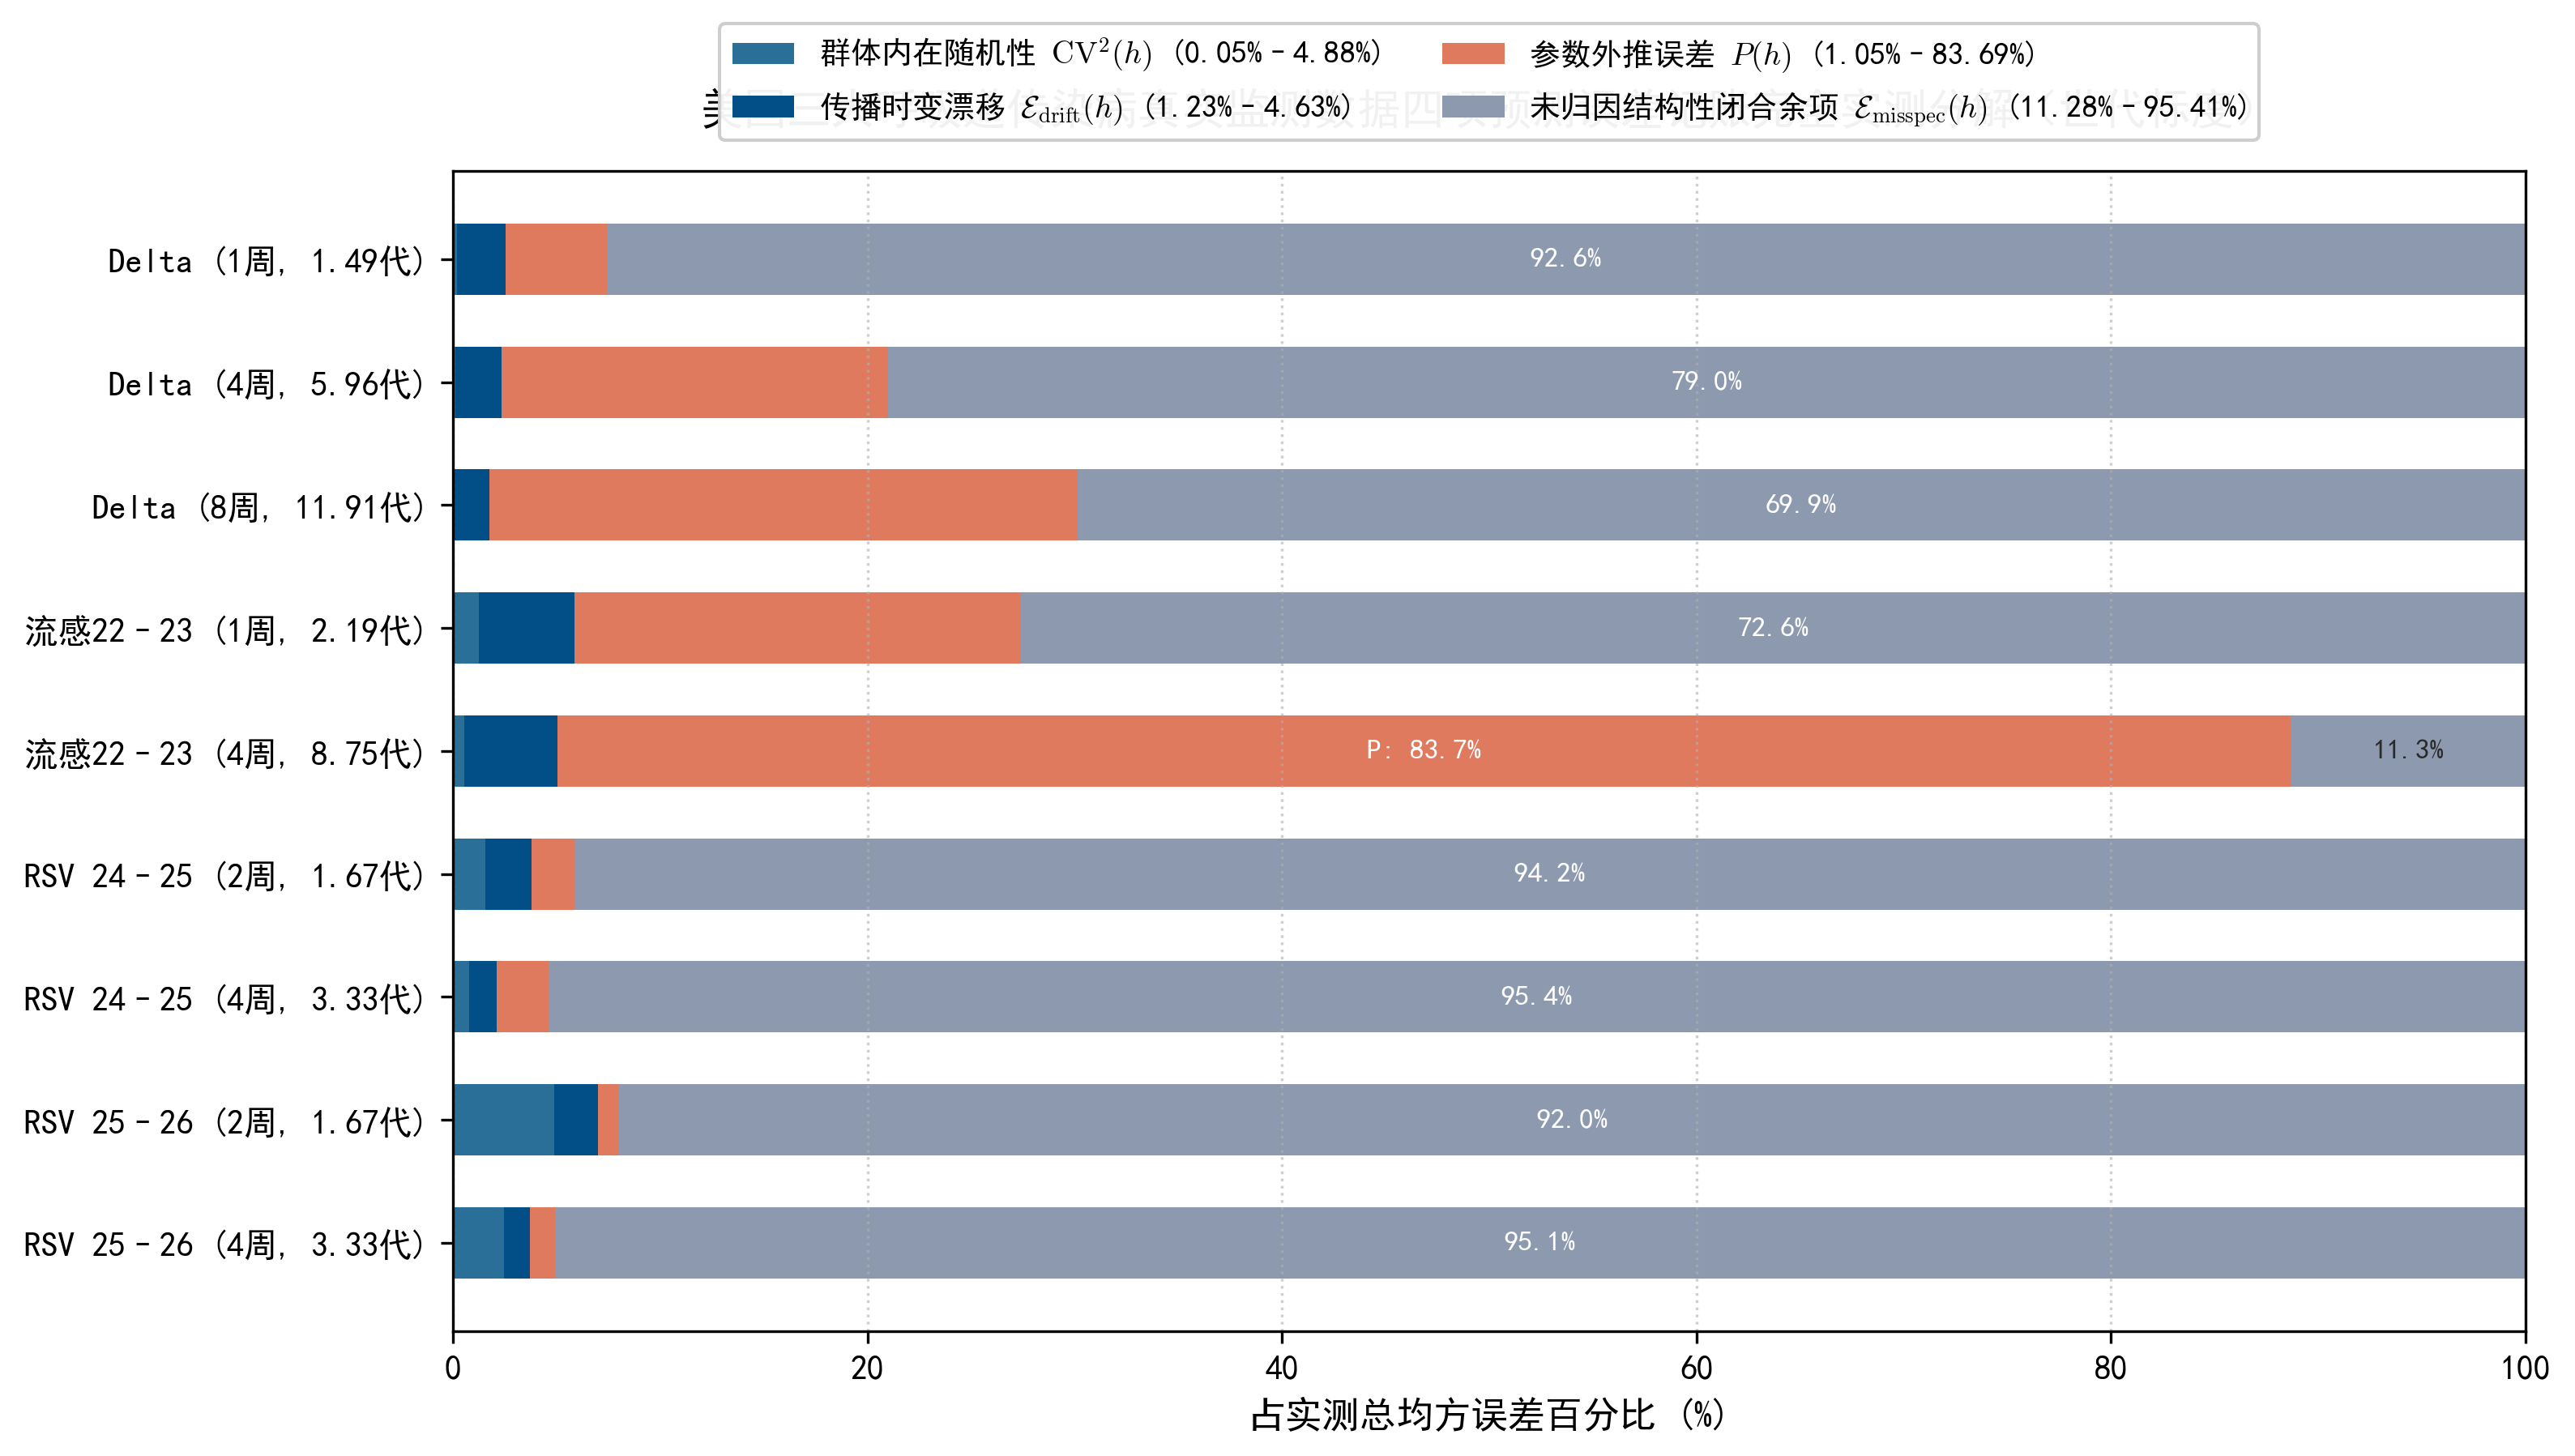
\includegraphics[width=\textwidth]{../reports/figures/fig6_error_budget.png}
\caption{Predicted error-budget decomposition across forecast horizons. Stacked bars show demographic floor (dark slate), $R$ fluctuation (cyan), and parameter uncertainty (orange) as percentages of total predicted variance. Budget shares shift toward parameter and $R$ components at longer horizons, while demographic floor dominates short-term forecasts.}
\label{fig:budget}
\end{figure}

Residual (realized minus predicted) requires further decomposition: beyond the three model components (demographic floor, $R$ drift, parameter uncertainty), the remainder is attributed to misspecification (e.g., generation-interval error, reporting delay, time-varying ascertainment). For COVID, the error-budget decomposition shows: at $h = 1$, the demographic floor accounts for 9.7\%, $R$ drift 7.6\%, and misspecification residual 82.8\%; at $h = 4$, floor 9.0\%, drift 7.0\%, misspecification 84.0\%; at $h = 8$, misspecification dominates ($\sim$86\%). The residual dominates even at short horizons, indicating that the constant-$R$ branching model's specification error for early COVID dynamics stems mainly from the rapidly changing transmission environment (variant emergence, behavioral response) rather than from parameter estimation itself; this decomposition makes the three-term attribution framework operational in practice---short-horizon failures should first prompt a check of model specification, while long-horizon failures implicate both $R$ drift and specification error.

Scaling exponents $p$ from log-variance $\sim h^p$ fits: COVID 1.13, influenza 1.00, RSV 0.48. The compatibility of these observed values with Theorem 5R requires care. The AR(1) persistence formula of Theorem 5R gives variance $\sim \gamma_0 h (1+\phi)/(1-\phi)$, i.e., $p \approx 1$---this corresponds to $\phi$ close to but slightly below 1 (strongly persistent growth, as COVID and influenza weekly growth rates have high autocorrelation, with $\phi$ estimated in 0.8--0.95). The $p = 3$ random-walk limit is approached only as $\phi \to 1$ over very long observation windows; the finite-length weekly data here cannot reach that limit. RSV's $p = 0.48 < 1$ corresponds to smaller $\phi$ (smoother growth, weak autocorrelation) or to smoothing in the processed series, under which variance grows sublinearly. Thus the observed scaling $p \in (0.5, 1.2)$ is consistent with Theorem 5R across different persistence parameters, not contradictory; the $p = 3$ limit is unreachable on the time scale of these data. Note that an exponent $p \approx 1$ is also what the population-level $1/k$ noise floor (Section~
\ref{eq:pop_floor}) predicts on its own, so the scaling exponent alone cannot distinguish "persistent drift" from "noise floor" as the mechanism; the error-budget amplitude decomposition (Figure~\ref{fig:budget}) is what separates the two. This is itself an instance of the paper's identification theme: a structural limit on what a single diagnostic (here, the log-variance exponent) can certify from data.

\begin{figure}[htbp]
\centering
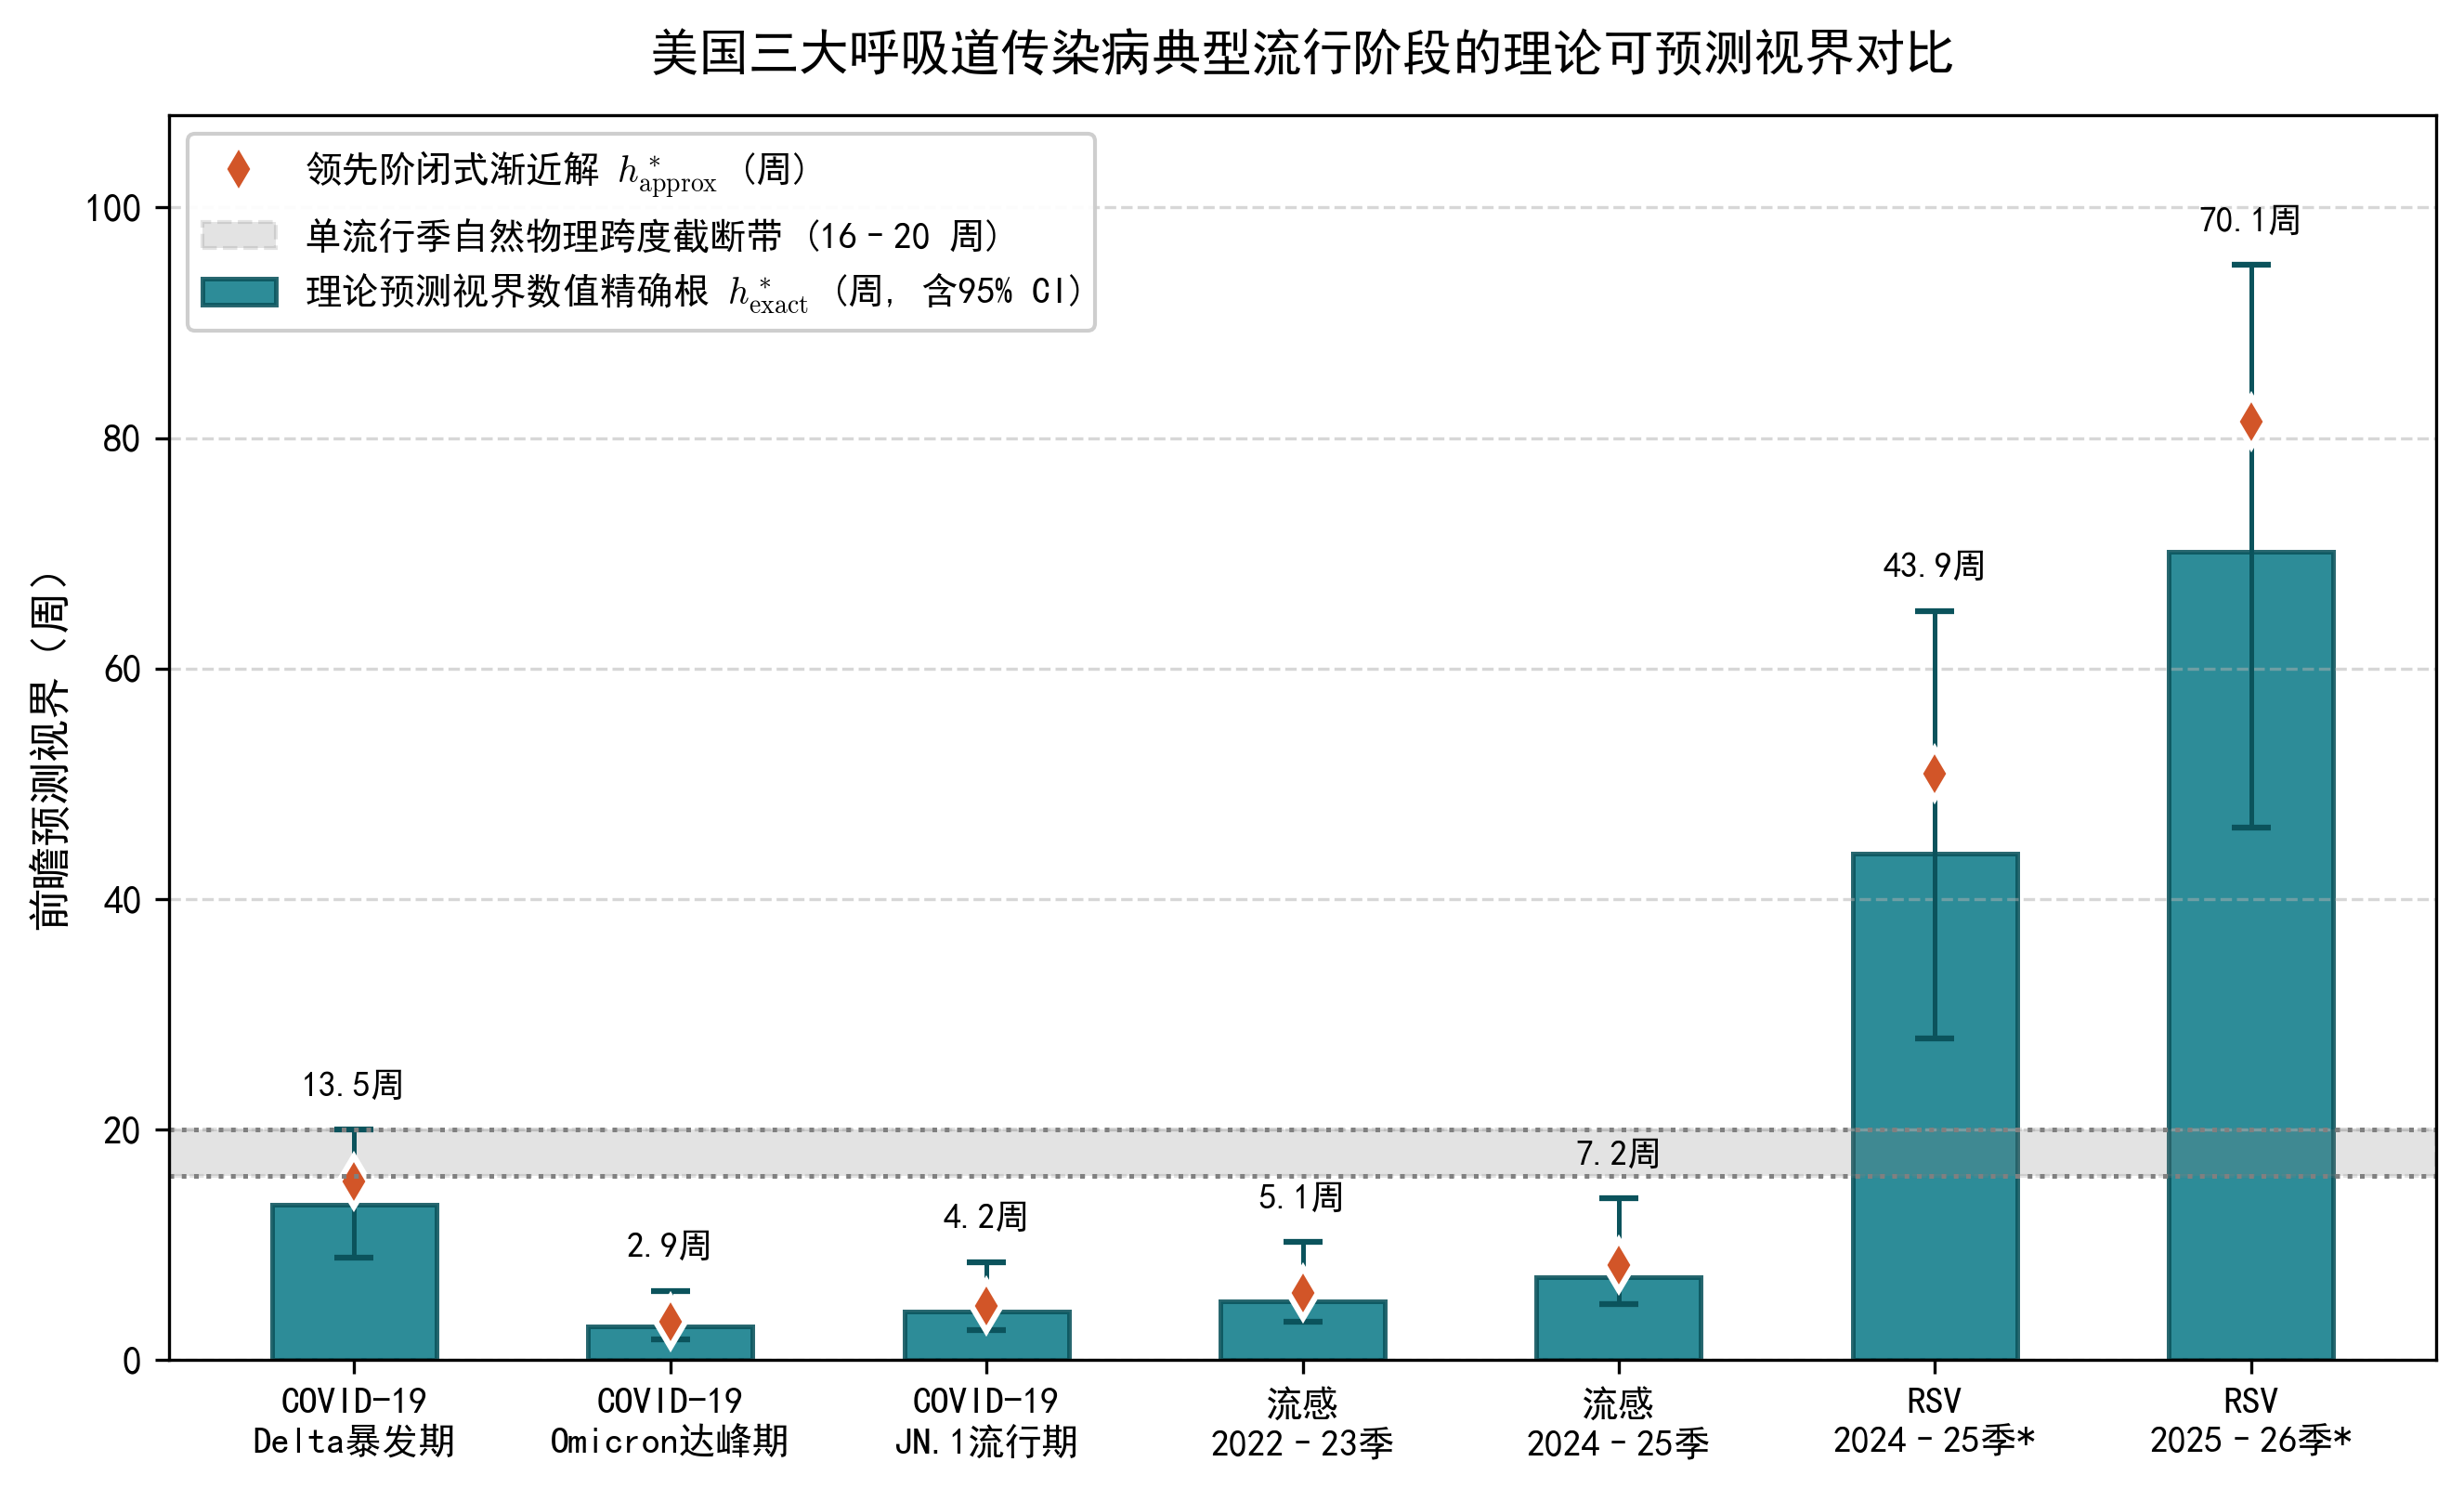
\includegraphics[width=0.75\textwidth]{../reports/figures/fig4a_real_horizons.png}
\caption{Real-data predictability horizons. Illustrative constant-$R$ horizons $h^*$ (weeks) for national COVID-19, RSV, and influenza phases from Table~\ref{tab:horizons} (2021--2025 surveillance windows). Horizontal bars show point estimates with 95\% bootstrap confidence intervals. The largest horizons (RSV 2025--26: 54.0 weeks) arise from the most precise $R$ estimates; phases with $R<1$ (COVID Omicron peak, Flu 2022--23 peak) yield $h^*=0$.}
\label{fig:real_horizons}
\end{figure}


\section{Discussion}

Epidemic predictability has a structural ceiling determined by $R$, $k$, scale, parameter precision, and noise model. Forecasting methods can approach this ceiling but cannot surpass it under the specified conditions. The practical interpretation is a forecast budget: resources should be allocated to phases where $h^*$ is positive and the three-term model accounts for observed error. Near-critical phases ($|\varepsilon| \ll 1$) and pre-onset periods ($R<1$) are information-theoretic blind zones; the correct response is to recognize the constraint and defer forecasting, not to demand accuracy where it is impossible. This reframing has a direct operational analogue in the RAPIDD Ebola challenge, where no participating model reliably beat a naive baseline in the low-incidence, near-extinction regime \citep{viboud2018rapidd}: our results suggest this was not a failure of modeling skill but an instance of $h^*\approx 0$, i.e., the near-critical window predicted by Theorem 3 and the finite-horizon boundary of Theorem 2. Broader reviews of operational forecasting during real outbreaks reach a similar qualitative diagnosis without a corresponding closed form \citep{funk2018realtime, held2017probabilistic, desai2019realtime}; the present theorems supply that missing closed form, and in doing so convert an empirical observation ("models struggle near threshold") into a falsifiable quantitative prediction ("models cannot do better than $h^*(R,k,I_0,\delta R)$").

The population-level $1/k$ floor implies that overdispersion limits predictability regardless of epidemic size, a consequence fundamentally distinct from sampling noise. This connects to a long-standing debate in disease ecology over whether population thresholds for invasion or persistence are a reliable organizing concept for control policy \citep{lloydsmith2005should}: our results indicate that even when a deterministic threshold nominally exists, the width of the near-critical window over which that threshold is operationally meaningless scales with $(R+1)/N$ and with $1/k$, so threshold-based decision rules inherit the same predictability ceiling as point forecasts. The critical slowing-down and long-tailed extinction-time behavior underlying Theorem 3 is the epidemiological instance of a more general phenomenon documented for critical stochastic spreading processes, including the classical analogy between the general epidemic process and dynamical percolation \citep{grassberger1983critical}.





The forecast-budget framing connects directly to standardized forecast-evaluation practice: interval-format scoring \citep{bracher2021evaluating} and multi-model ensemble comparisons \citep{cramer2022evaluation} could incorporate $h^*$ as a pre-registered ceiling, flagging phases where further model refinement cannot be expected to improve scores. In practice, this suggests reporting $h^*$ alongside every operational forecast: a forecast issued at $h>h^*$ is not merely less accurate but is, under the stated assumptions, attempting to resolve information that the data-generating process does not contain at that lead time. This is a stronger and more falsifiable claim than the qualitative "forecasts are less reliable early in an outbreak" that pervades the applied forecasting literature \citep{desai2019realtime}.



\subsection{Implications for public-health communication}

The horizon $h^*$ has a direct analogue in risk communication: rather than issuing a single point forecast with wide confidence intervals that mask the underlying structural constraint, public-health dashboards could present $h^*$ as a time boundary separating "predictable" from "inherently noisy" phases. This reframing addresses a recurring tension in outbreak communication: decision-makers often request precise forecasts during the early, high-uncertainty phase of an outbreak, precisely when $h^*$ is shortest \citep{viboud2018rapidd, funk2018realtime}. Reporting $h^*$ explicitly provides a defensible, quantitative basis for declining to issue long-horizon forecasts rather than issuing them with caveats that are easily overlooked. For example, during the COVID-19 Delta wave (Jul 2021), our illustrative $h^* = 17.3$ weeks (95\% CI [11.8, 41.6], $\approx 4.5$ months) indicates that 6-month forecasts exceed the predictable regime under constant-transmission assumptions, whereas the Omicron peak (Jan 2022) with $R < 1$ yields $h^* = 0$, signaling that any forward projection is dominated by noise and near-critical uncertainty. The confidence intervals themselves communicate parameter-estimation uncertainty; when the lower bound of the CI includes zero, the message is unambiguous: "current data do not support a positive predictability horizon." This is operationally distinct from issuing a forecast with wide intervals, which can give the false impression that a precise forecast is possible but merely requires better data; the $h^* = 0$ verdict instead says the limitation is structural, not data-quality-dependent.

A related implication concerns multi-model ensemble forecasting hubs \citep{mcgowan2019collaborative, reich2019collaborative, cramer2022evaluation}, which aggregate submissions from diverse modeling teams. Ensembles typically outperform individual models \citep{ray2020ensemble}, but our results suggest this aggregation cannot push ensemble performance beyond $h^*$: if the bound is set by the data-generating process rather than by any single model's specification, then ensemble averaging reduces model-specific misspecification error but does not remove the intrinsic noise captured by the demographic floor and the parameter-uncertainty term. This prediction is testable: ensemble forecast skill should plateau or degrade sharply as $h \to h^*$, a pattern that has been observed qualitatively in FluSight and COVID-19 Forecast Hub retrospectives \citep{mcgowan2019collaborative, cramer2022evaluation} but not yet formalized as a pre-registered hypothesis keyed to a mechanistic bound. Incorporating $h^*$ into hub evaluation protocols would make this test explicit.

The machine-learning results clarify the value of adaptive methods: ML-2 shows strong learners saturate the bound; ML-1 shows neural estimators do not cross the identification floor under correct likelihood specification \citep{lehmann1998theory}. The ML-1 result also delineates where flexible, mechanism-agnostic models such as those used for clinical or case-level Ebola prediction \citep{colubri2019machine} are likely to add value: not by beating a correctly specified mechanistic estimator on parameters the mechanism already captures, but by absorbing structure (reporting artifacts, heterogeneous risk groups, covariates) that the branching-process likelihood does not model at all.

\subsection{Relation to deterministic threshold theory}

Our stochastic framework complements rather than replaces classical deterministic epidemic threshold theory \citep{kermack1927contribution, anderson1991infectious}. In large, well-mixed populations, the law of large numbers implies that the branching process converges to the deterministic SIR/SEIR system, and the basic reproduction number $R_0$ serves as a sharp invasion threshold: $R_0 > 1$ guarantees an outbreak, $R_0 < 1$ guarantees extinction. However, this sharp threshold is a large-$N$ limit that ignores two sources of uncertainty central to our results: demographic stochasticity (individual-level offspring variation) and parameter uncertainty (imperfect estimation of $R$ and $k$ from finite data). Theorem 3 quantifies the first effect: even in the limit of perfect parameter knowledge, the near-critical window $|R - 1| = O(1/N)$ exhibits quasi-stationary fluctuations with a large coefficient of variation (0.132 at $(\varepsilon,R,N)=(0.2,1.2,2000)$ and 1.67 inside the window at $(\varepsilon,R,N)=(0.005,1.005,2000)$, i.e., relative error of order the mean itself; the quasi-stationary density of Theorem~3(a) is verified empirically in both regimes, ratios 0.998--0.999 and 0.976) and long-tailed extinction times $\sim N^{1/2}$, so the deterministic threshold is operationally blurred over a window whose width is inversely proportional to population size. For human respiratory pathogens with effective population sizes $N \sim 10^3$--$10^5$ \citep{ethier1986markov, bettencourt2008real}, this window spans $R \in [0.998, 1.002]$ to $[0.99998, 1.00002]$ (from $(R+1)/N \approx 2/N$ at $R \approx 1$), meaning that the yes/no invasion question remains unresolved for weeks to months even when $R$ is known exactly.

Theorem 4 adds the second layer: in realistic surveillance settings, $R$ is estimated from finite cumulative incidence, and the Cramér-Rao bound implies that distinguishing $R = 1.0$ from $R = 1.1$ requires cumulative case counts $\gg k(R + 1/R) \approx 2k$ when $R \approx 1$. For highly overdispersed pathogens ($k \sim 0.1$, e.g., early SARS-CoV-2 \citep{endo2020overdispersion, adam2020clustering}), this threshold is modest ($\sim 0.2$ cases), but the finite-sample MLE efficiency loss (ratio 0.57--1.81 in our simulations) means that operational $R$ estimates remain noisy even after hundreds of cases. The practical upshot is that the deterministic $R_0 = 1$ threshold, while theoretically exact in the $N \to \infty$ and perfect-information limits, is surrounded by a predictability desert in both directions: stochastic fluctuations dominate when $N$ is finite (Theorem 3), and parameter noise dominates when cumulative incidence is small (Theorem 4). Our finite-horizon formulas (Theorems 1, 2) synthesize these two effects into a single operational criterion\textemdash the predictability horizon $h^*$\textemdash that decision-makers can evaluate from real-time data without requiring asymptotic limits.

What the limits do and do not say. Read together, the theorems give surveillance systems concrete numbers rather than vague warnings. Theorem 1: a forecast issued beyond $h^*$ is attempting to resolve information the process does not contain at that lead time; for the illustrative COVID Delta phase ($R=1.31$, $\delta R=0.028$, $\tau=0.5$) this boundary is 17.3 weeks (4 months), so a 6-month deterministic projection is not merely risky but structurally unsupported. Theorem 3: the near-critical window has width $\sim (R+1)/N$; at effective population size $N=10^3$ the yes/no invasion question is unresolved inside $R \in [0.998, 1.002]$, and the window narrows only as $1/N$. Theorem 4: deciding $R>1$ needs cumulative incidence of order $(1/R+1/k)/\varepsilon^2$ (about 200 cases at $R=1.1$, $k=1$, rising to roughly $10^3$ with a 0.05-significance, 0.8-power test). These limits do not imply that early-warning systems are useless; as Drake argued for epidemic early-warning precision \citep{drake2005fundamental}, they define what it is reasonable to expect from a given surveillance investment. Timing and average-size forecasts can still be valuable even when the final size or the exact regime is not resolvable at the target accuracy; the limits identify which forecast products are worth building for which phase, not a blanket prohibition on forecasting near threshold.

This synthesis clarifies a persistent ambiguity in applied outbreak analysis: when an early-phase forecast fails (e.g., RAPIDD Ebola challenge \citep{viboud2018rapidd}), is the failure due to model misspecification (wrong transmission mechanism), data inadequacy (too few cases), or intrinsic unpredictability (the process is near-critical)? Deterministic threshold theory offers no quantitative criterion to distinguish these; our Theorem 1 decomposition does, attributing forecast variance to demographic floor (unavoidable even with perfect parameters and infinite $N$), parameter uncertainty (reducible by collecting more data), and $R$ drift (evidence of model misspecification). The real-data error-budget analysis (Figure~\ref{fig:budget}) operationalizes this: for COVID, the misspecification residual dominates at every horizon (82.8\% of the variance at $h = 1$, 84.0\% at $h = 4$, $\sim$86\% at $h = 8$), so short-horizon failures for that pathogen point first to model specification; for the more stable RSV 2024--25 wave, the three-term model accounts for 63\% of the variance at $h = 2$ and 77\% at $h = 4$ (and exceeds the observed variance at $h = 8$, where the residual is zero), indicating that the constant-$R$ branching-process assumption is a reasonable working model for that phase. Deterministic models cannot perform this attribution because they have no demographic-noise term.


\section{Limitations}


Several modeling assumptions and data-processing choices bound the scope of the results. Model assumptions. The theorems are proven for the generation-counting Galton-Watson model with negative-binomial offspring and constant $R$ over the horizon; the continuous-time renewal extension (Theorem 5R) employs a delta-method approximation. The constant-$R$ horizon is an ideal-case bound: real outbreaks exhibit $R$ drift from behavioral responses, variant emergence, and interventions, which are not captured by the branching-process model and which shorten the operational horizon relative to $h^*$. Relatedly, $h^*$ is an upper bound under the fitted model: when the fitted constant-$R$ family is misspecified, as the COVID error budget suggests it is even at short horizons (misspecification residual 82.8\% at $h=1$), the true process may have a ceiling below $h^*$; Theorems 5 and 5R handle drift partially, and the budget decomposition attributes the remainder. Theorem 4 is a likelihood-specific order-of-magnitude statement; the wide verification range (0.57--1.81) reflects MLE efficiency variation across parameter regimes rather than a tight bound. Theorem 3's small-$\varepsilon$ simulation is limited by finite mixing time of the quasi-stationary dynamics. Data-processing choices. Real-data $\hat{k}$ estimates are moment-based on 8-week moving windows; shorter windows are noisier (CV $>0.5$ at 4 weeks in low-incidence RSV phases), and longer windows smooth over genuine temporal variation in superspreading intensity. Table~\ref{tab:horizons} is illustrative, not a claim of operational forecasting superiority; the horizons assume finalized (non-nowcast) surveillance data and ideal constant-transmission conditions. The confidence intervals in Table~\ref{tab:horizons} rely on parametric bootstrap rather than the finite-sample, anytime-valid guarantees available from confidence-sequence methods \citep{howard2021time, shin2022edetectors, waudby2023estimating}; adapting these to the horizon estimator is a natural extension for sequential, streaming surveillance use.



\section{Conclusion}

We have characterized fundamental limits of epidemic predictability: a closed-form horizon with exact error decomposition, a finite-horizon accuracy boundary, a near-critical window with quasi-stationary density and establishment probability, a likelihood-specific identification floor, and a closed-form treatment of persistent growth-rate drift. Verification spans six theorems, machine-learning bound checks, and real-data decomposition. On data that exactly satisfy the mechanism assumptions, flexible learners saturate the theoretical bounds; their incremental value in realistic settings lies in capturing covariates and reporting artifacts that the branching likelihood leaves unmodeled. The contribution is not a claim of forecasting superiority but a precise delineation of where such superiority ends\textemdash an account of the possible, and the impossible.

This delineation has two intended uses. First, as a diagnostic: when an operational forecast underperforms near an epidemic threshold, the three-term decomposition (demographic floor, parameter uncertainty, $R$-drift) offers a first-pass attribution before invoking model misspecification or data quality as explanations, consistent with the recurring observation that near-threshold failure appears across very different modeling frameworks \citep{funk2018realtime, held2017probabilistic, viboud2018rapidd}. Second, as a design constraint: surveillance systems, dashboards, and forecasting hubs \citep{mcgowan2019collaborative, johansson2019open, cramer2022evaluation} could report $h^*$ alongside point forecasts and calibrated intervals, making explicit the horizon beyond which further precision cannot be expected under the stated process assumptions. Extending the theorems to structured populations, time-varying dispersion $k$, and reporting delay is left to future work; each is a natural relaxation of assumptions (A1)--(A4) and would sharpen the boundary for settings\textemdash spatial heterogeneity, superspreading dynamics \citep{lloydsmith2005should}, and evolving surveillance systems\textemdash where the present constant-parameter treatment is only a first approximation.


\bibliographystyle{elsarticle-num}
\bibliography{references}

\end{document}